\chapter{Classroom Case Study}
\label{ch:Classroom}
Following the pilot study and collaborative research with Dr. Hakan Erdogmus\footnote{Dr. Hakan Erdogmus is a Senior Research Officer in the NRC-IIT Software Engineering Group (http://iit-iti.nrc-cnrc.gc.ca/personnel/erdogmus\_hakan\_e.html). He has interests in Software Economics, Agile Software Development, and Software Process Measurement and Awareness.},  I improved Zorro and conducted an extended validation study in the software engineering classes at the University of Hawaii in Fall 2006. This study shows that Zorro can collect low-level development activities and infer TDD development behaviors accurately. This study also provides evidence that Zorro is helpful for beginners who do not have much prior experience with the TDD practice. 

\begin{comment}
The classroom case study is an evaluation designed to evaluate Zorro's low-level development activity collection and automated inference of Test-Driven Development behaviors. This chapter has three sections. Section \ref{sec:CaseStudyMethod} explains the analysis method for individuals using the first participant's data. Section \ref{sec:CaseStudyFindings} presents the summary of analysis results over all participants' data. In the end Section \ref{sec:discussion} discusses the research findings from this research. The pilot study of Zorro was a success. It convinces us that Zorro's rule-based approach has promise for developer's TDD behavior inference. It also demonstrates that the research methodology works. Following this study, I fixed several data collection problems found in the pilot study. We also improved Zorro's TDD inference rules based on the pilot study and collaboration with Software Engineering Group at the National Research Council of Canada.
\end{comment}

\section{Purpose of the Study}
The purpose of this study was to validate Zorro using the case study research method tested by the pilot study (Chapter \ref{ch:Pilot}) and investigate how useful Zorro is for TDD beginners. 

\begin{comment}
Currently Zorro collects development activity data more accurately,
has a more sophisticated episode classification schema, and infers
developer TDD behaviors based not only on the episode's internal
structure but also the context in which the episode occurred.
The purpose of this study is to:
\begin{enumerate}
\item perform Zorro validation study using the Eclipse Screen Recorder;
\item perform a second type of validation in which participates
provide feedback through the web-based validation wizard of Zorro;
\item obtain feedback regarding whether Zorro can help TDD
beginners through a post-test interview.
\end{enumerate}
\end{comment}

\section{Research Questions}
The specific research questions for the classroom case study were:
\begin{itemize}
\item{Q2a: Does Zorro collect software development activities accurately enough for episode partitioning and TDD behavioral inference?}
\item{Q2b: Does Zorro's inference of TDD behaviors agree with analyses based upon participant observation?}
\item{Q2c: Does Zorro's inference of TDD behaviors agree with what participants believe to be their TDD behaviors?}
\item{Q2d: Does Zorro provide useful information for beginners to understand TDD and improve their TDD development?}
\end{itemize}

Research questions Q2a, Q2b, and Q2c are three specific research questions for the thesis research question Q1, ``\textit{Can Zorro automate the recognition of TDD behaviors using automatically collected software metrics?}''. The research question Q2d corresponds to the thesis research question Q2, ``\textit{How useful is Zorro?}'' 

\section{Experiment Design}
\label{sec:ClassroomDesign}
To address the above research questions, I used the one-shot case study research method as in the pilot study. TDD was the treatment. We taught TDD to participants and asked them to develop software using TDD in this study. 

\subsection{Participants}
TDD beginners were the targeted population. I recruited participants from a senior-level software engineering class and a graduate-level software engineering class, both of which were taught by Professor Philip Johnson in Fall 2006 at the University of Hawaii. There were 16 students in two classes and 11 of them agreed to participate in this study. 

\subsection{Materials}
I conducted this study in the Collaborative Software Development Laboratory (CSDL) at the University of Hawaii. Three Windows-based lab computers were used, one of them acted as a Hackystat server and the other two were used by participants to develop software for this study. I configured two development computers with necessary software including JDK, Eclipse, the Hackystat Eclipse Sensor, QuickTime and ESR. Bowling Score Keeper, a famous problem that has been widely used in empirical evaluation research of TDD\cite{George:03,Erdogmus:05}, was the programming task. Since participants were TDD beginners, I designed user stories in plain text (Appendix \ref{app:UserStoriesBSK}) to help them develop the program without needing prior experience with the game. Since user stories are ordered from the easiest one to the hardest one, they can also be used as the ``To Do'' list for TDD development.  

\subsection{Instruments}
I instrumented the development processes with the Hackystat Eclipse sensor and ESR. Prior to the study, I created a Hackystat key for each participant and configured the Hackystat Eclipse sensor for him/her. At the beginning of the study, I asked participants to enable ESR so that it would record their development processes. Participants validated Zorro's TDD behavioral inference using the ``TDD Episode Validation'' (Figure \ref{fig:EpisodeFeedback}) analysis. The ``Web Validation Wizard'' was another instrumentation tool that I used to collect participant's evaluation. Additionally I interviewed participants in the study and recorded the interviews using a digital voice recorder.

\subsection{Procedure}

This experiment included a TDD lecture and a 2-hour lab session. 

\begin{enumerate}
\item{TDD Lecture}

In both software engineering classes, Professor Philip Johnson gave the same TDD lecture to students. The lecture included following contents:
\begin{itemize}
\item Introduction to TDD
  \begin{itemize}
  \item Two principles of TDD from \cite{Beck:03}
  \item Red/green/refactor pattern of TDD
  \item TDD Rhythm \cite{TDDRhythm}
  \item TDD vs. Unit Testing
  \item A TDD example: implementing stack by writing test first 
  \end{itemize}
\item Why TDD?
  \begin{itemize}
    \item{Developer gets quick feedback.}
    \item{TDD improves software quality.}
    \item{TDD promotes simple design.}
    \item{Microsoft has successful story on TDD \cite{Bhat:06}}
    \item{Test-Driven Development proves useful at Google\cite{RoyOsheroveBlog}}
  \end{itemize}
\item About TDD
  \begin{itemize}
    \item{TDD may not be appropriate for everybody.}
    \item{TDD is about design.}
    \item{Some studies show that TDD improves software quality.}
    \item{TDD may reduce productivity.}
    \item{TDD references including testdriven.com, mailing list and blogs.}
  \end{itemize}
\item Reading and programming assignments
  \begin{itemize}
    \item {Page 1-20 of Beck's book ``Test-Driven Development by Example'' \cite{Beck:03}}
    \item {TDD Quick Reference \cite{TDDQuickReference}}
    \item {Practice TDD on Roman Numeral Problem (Appendix
    \ref{app:UserStoriesRomanNumeral})}
  \end{itemize}
\end{itemize}

After the lecture, students practiced TDD by working on an in-class assignment, the Roman Numeral Conversion (Appendix \ref{app:UserStoriesRomanNumeral}). Then they were asked to voluntarily participate in this study. The study was conducted in CSDL under my supervision. The 2-hour lab session included 90-minute of development using TDD, Episode Validation, Participant Interview and Zorro Usefulness Evaluation. 

At the beginning of the study, I introduced the purpose and content of this research study to participants, followed by the consent form signing. Then I gave them user stories of the Bowling Score Keeper problem (Appendix \ref{app:UserStoriesBSK}) and explained that they only needed to spend 90 minutes on the programming task. Following a five minute introduction, I asked them to start up Eclipse, enable the ESR recorder and begin programming. 

\item{TDD Development (90 minutes)}

Each participant developed a program to compute bowling game scores in TDD following the provided user stories. I suggested that they use the user stories as a To-Do list to help them develop in TDD. The time limit was 90 minutes. It was acceptable if they did not finish all user stories by the end within the 90 minutes. 

\item{Validating Zorro's Inference about Their TDD Behaviors (15 minutes)}

After 90 minutes of development in TDD, participants exited Eclipse, which forced the Eclipse sensor to send all remaining development activities to the Hackystat server and stopped the ESR recorder. Following a five minutes coffee break, I then directed them to login into the Hackystat server and asked them to invoke the ``TDD Episode Validation'' (Figure \ref{fig:EpisodeFeedback}) analysis in which they provided their feedback to Zorro's inference results. As seen in Figure \ref{fig:EpisodeFeedback}, they commented on Zorro's inference of development behaviors and compliance to TDD. 

%they will use the Zorro evaluation wizard to analyze their TDD development and validate Zorro's TDD behavior inference (Figure \ref{fig:EpisodeFeedback}).

\item{Interview (5 minutes)}

I conducted an interview with each participant after he/she finished reviewing Zorro's inference of their development behaviors. The interview lasted 5 minutes. In the interview, I asked  participants questions regarding their development experiences on software engineering best practices, unit testing, TDD and software quality. 

\item{Zorro Usefulness Evaluation (10 minutes)}

At the end of the lab session, participants conducted several analyses using the ``Evaluation Wizard'' (Figure \ref{fig:EvaluationWizard}) provided by Zorro to evaluate its usefulness. 
\begin{figure}[htbp]
  \centering
  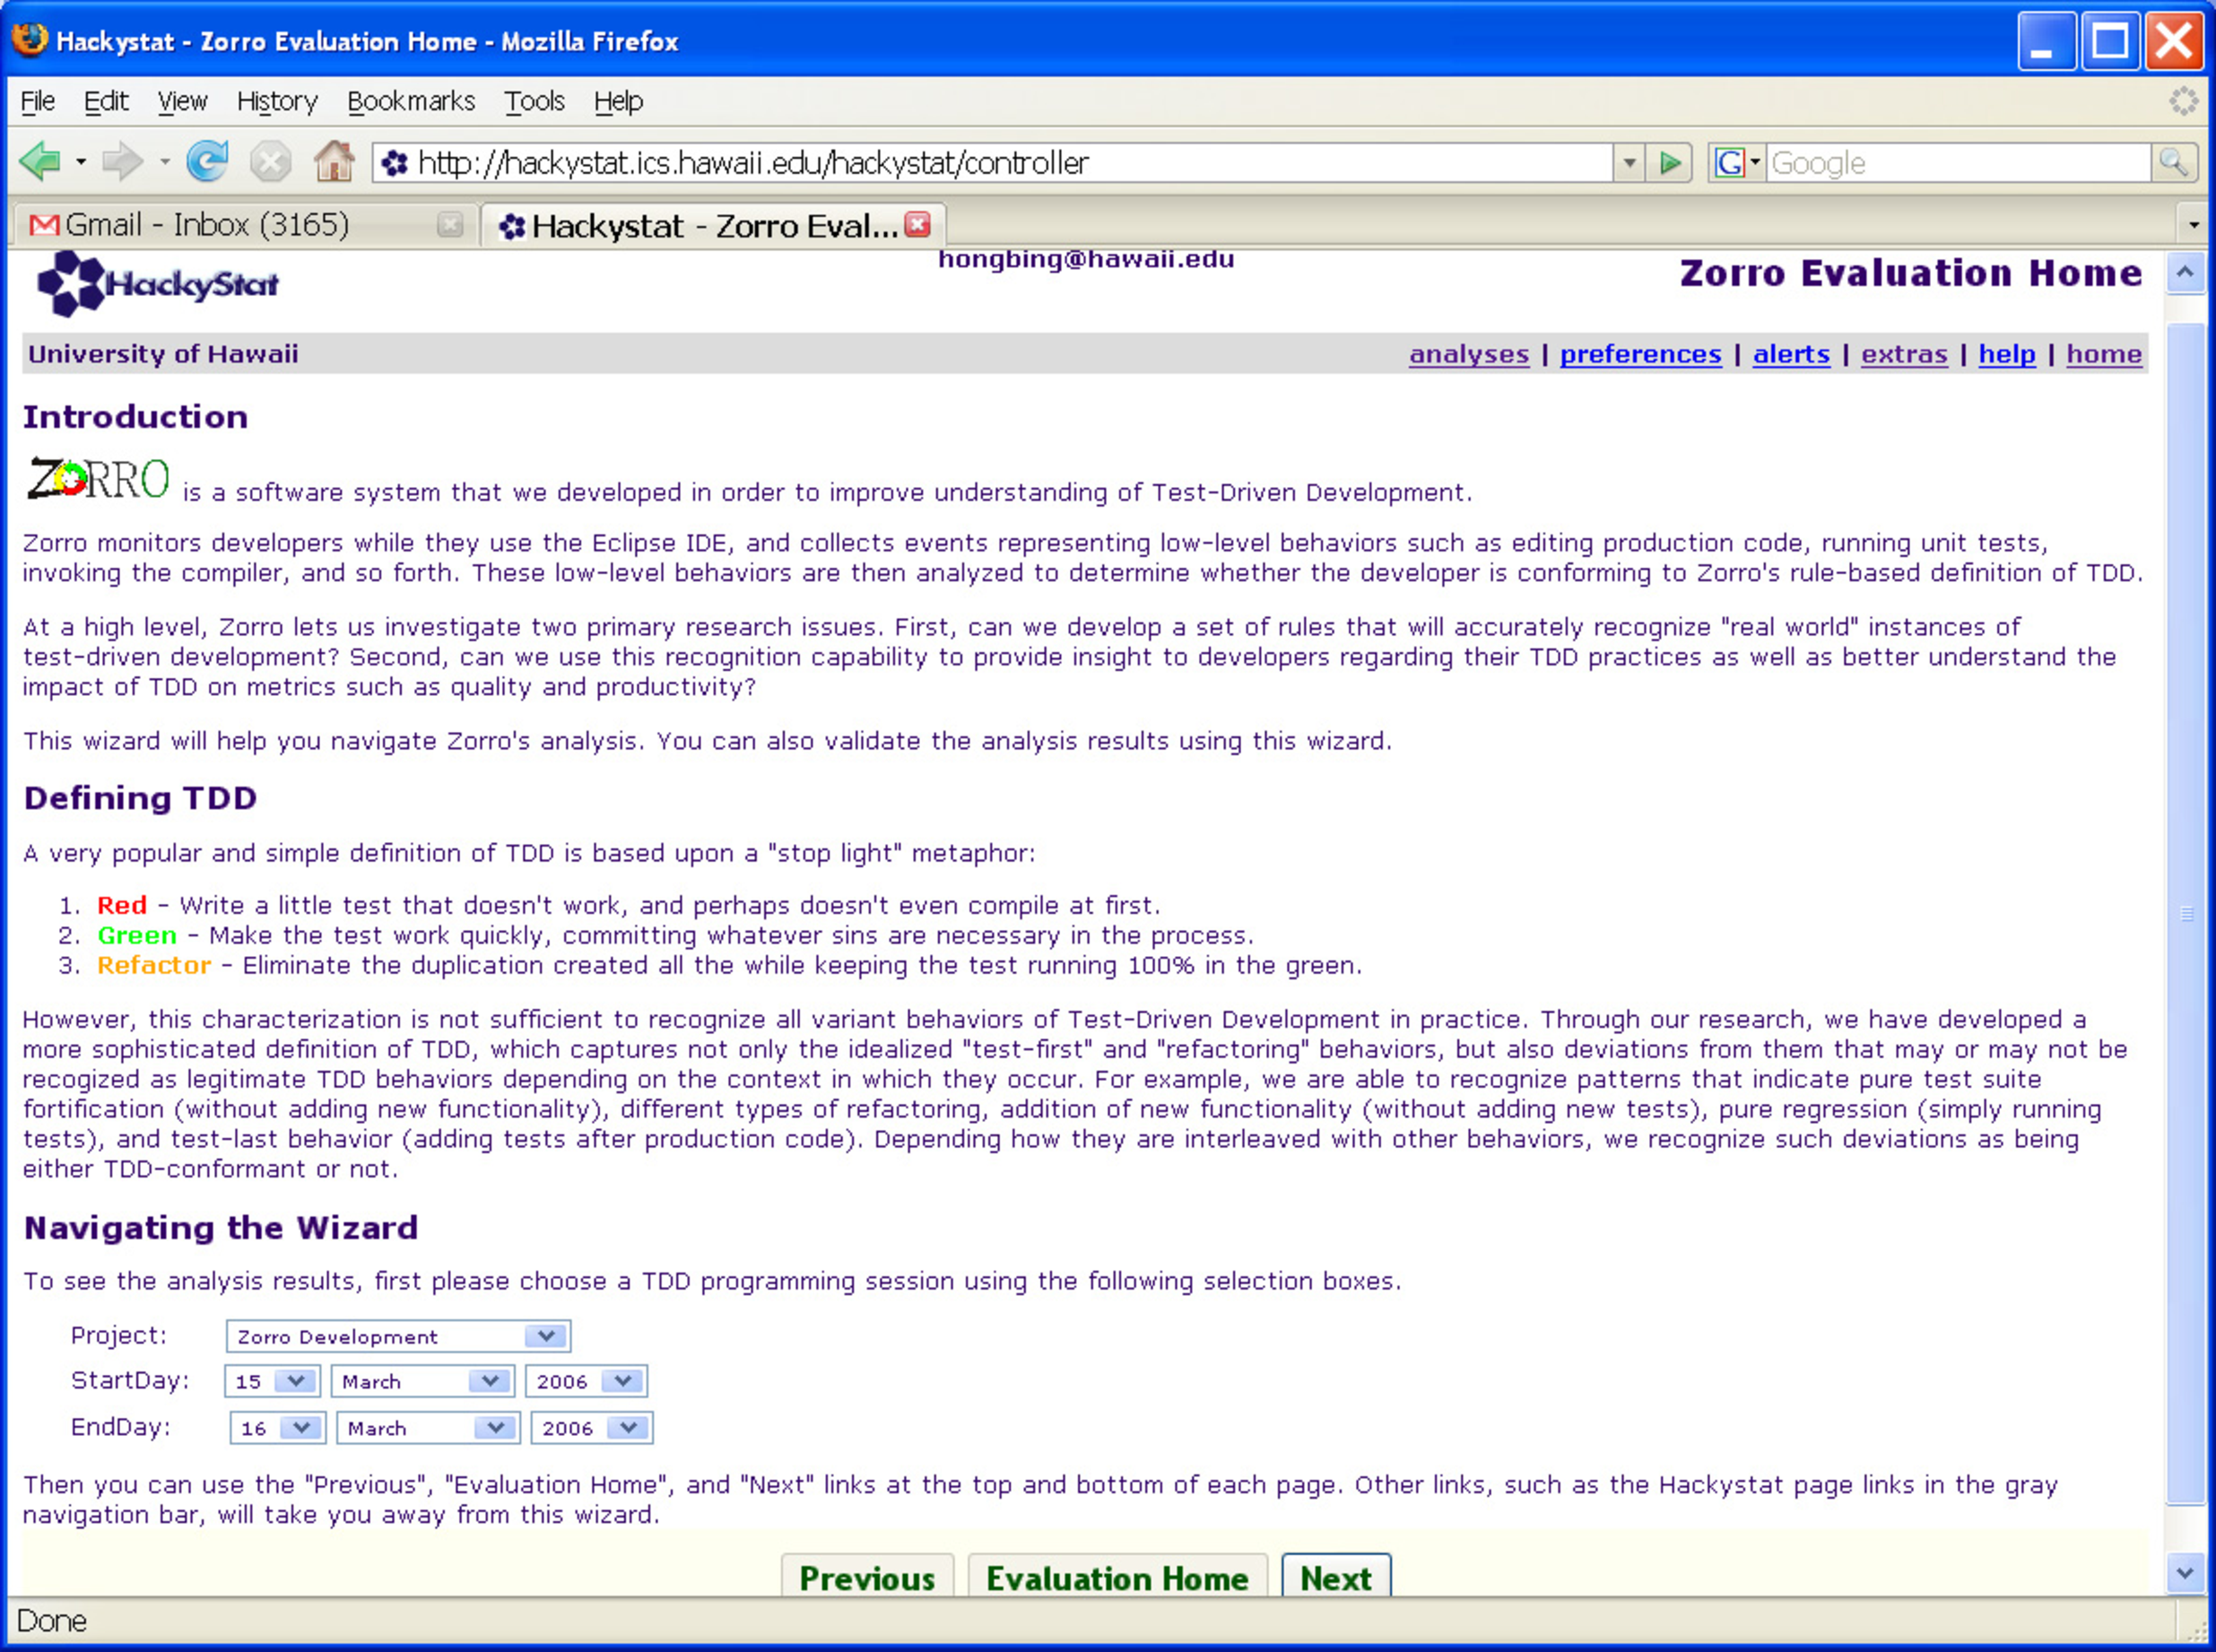
\includegraphics[width=0.8\textwidth]{figs/EvaluationWizard}
  \caption{Zorro Evaluation Wizard}\label{fig:EvaluationWizard}
\end{figure}
Participants used the wizard to review five analyses that were created based on Zorro's inference: Episode Demography, T/P Effort Ratio, T/P Size Ratio, Episode Duration and Episode Duration Bin. 

%, each participant took a 5 minutes coffee break before the interview started. The interview lasted 15 minutes during which I asked questions regarding the participant's experiences and opinions on unit testing, TDD and software quality. 

%In the end I will interview participants. The purpose of this interview is to learn participant's opinions on unit testing and TDD, discover questions and problems they may have, and investigate whether and how Zorro can help TDD beginners. The interview protocol and outline are available at Appendix \ref{app:CaseStudyInterviewGuide}.

\end{enumerate}

\subsection{Data Collection}
\label{sec:Classroom-DataCollection}
Similarly to the pilot study, I collected development activities using the Hackystat Eclipse sensor and development process videos using ESR. Development activities were saved on the Hackystat server, and ESR videos were saved on the lab PCs. To collect participants' validation comments, Zorro provides the ``TDD Episode Validation'' analysis (Figure \ref{fig:EpisodeFeedback}), which is an extension to the ``TDD Development Stream'' analysis (Figure \ref{fig:gui}) discussed in Section \ref{sec:Pilot-Analysis}. 
\begin{figure}[htbp]
  \centering
  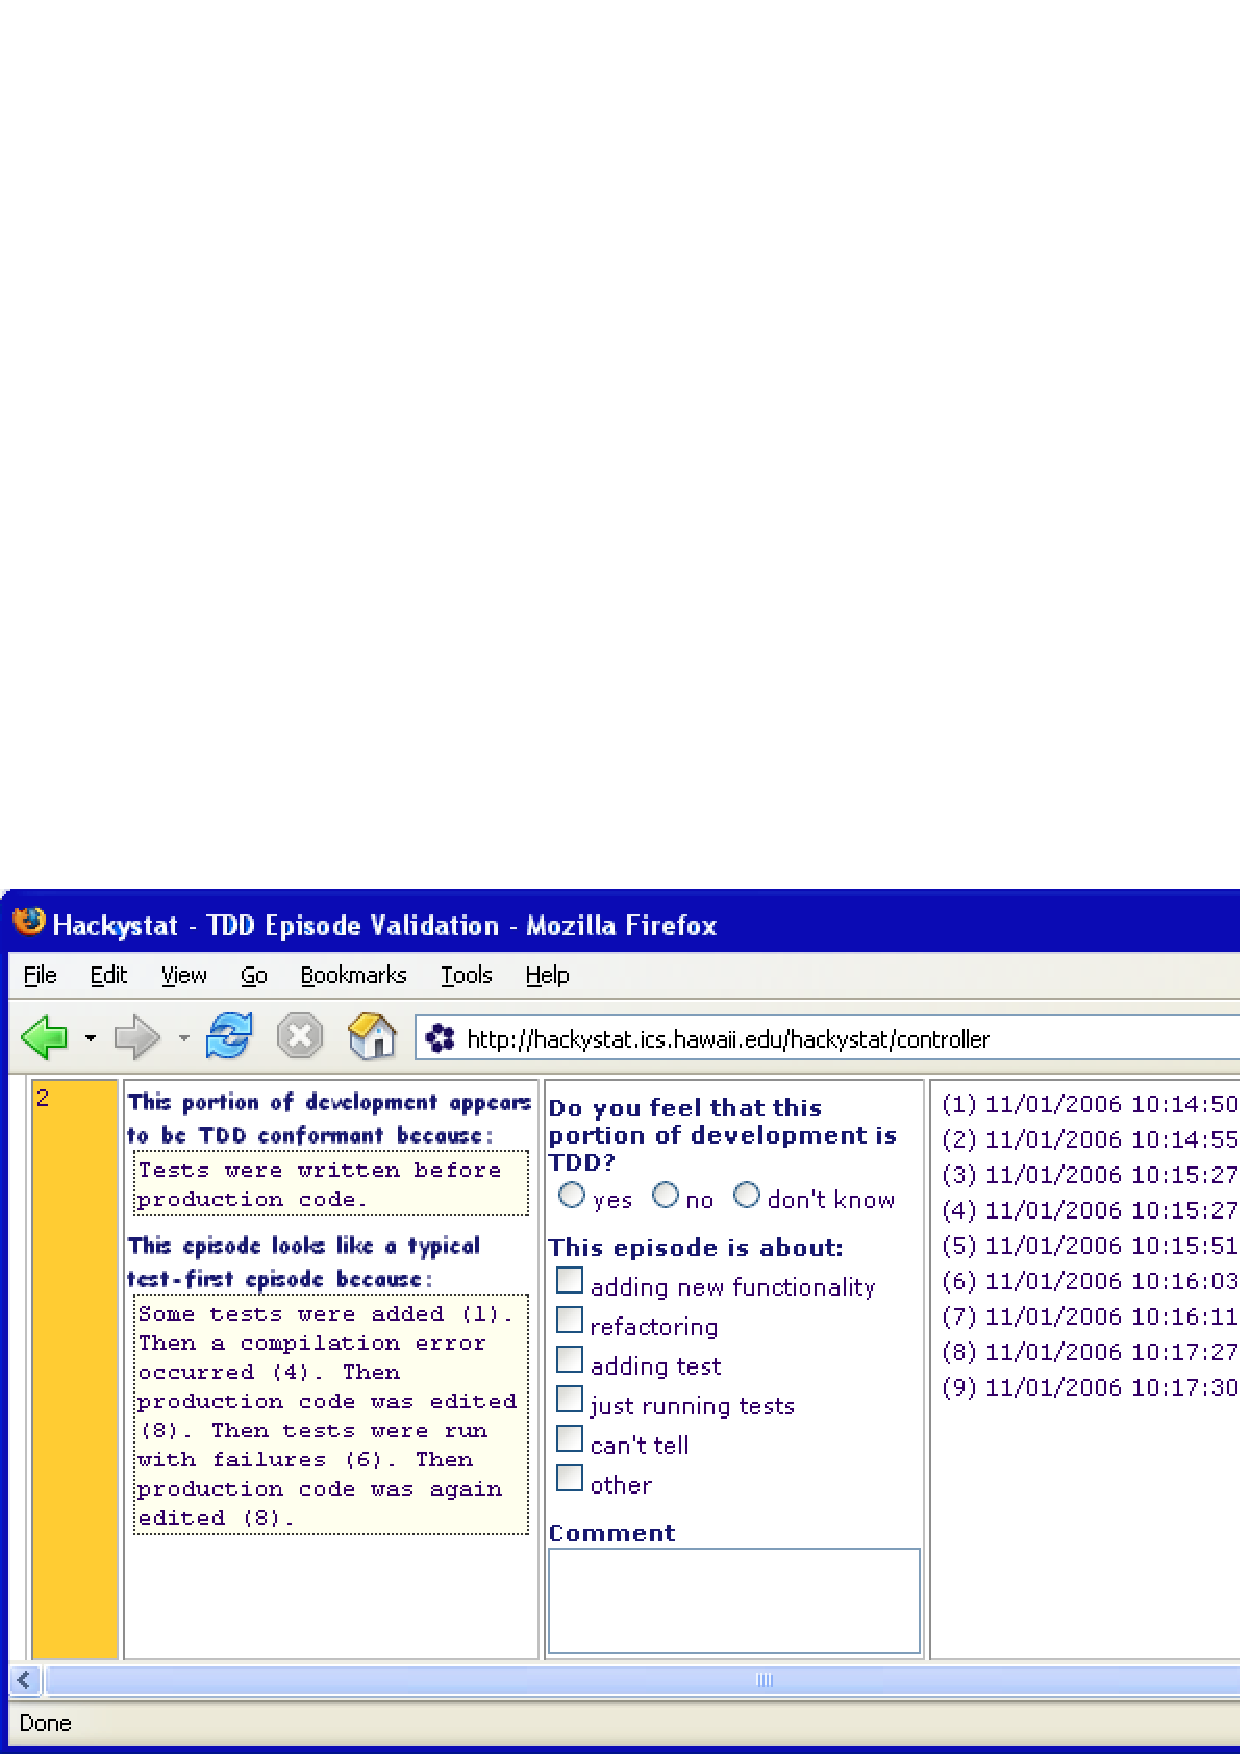
\includegraphics[width=1.0\textwidth]{figs/EpisodeFeedback}
  \caption{TDD Episode Validation}\label{fig:EpisodeFeedback}
\end{figure}
In addition to presenting inference results, this analysis also supplies Zorro's reasoning process and allows participants to give feedback, which was saved to the Hackystat server. Participants conducted Zorro usefulness evaluation using the ``Evaluation Wizard'' analysis (Figure \ref{fig:EvaluationWizard}) that saved the evaluation results to the Hackystat server too. 

%an episode validation analysis for users. This analysis presents Zorro's TDD behavior inference and the underlying reasoning process. It provides three choices for participants to indicate whether they agree or not with Zorro's inference on their TDD development behaviors. In the same analysis, they can also use a set of check-boxes and a text-box to provide additional information about their actual  development behaviors (Figure \ref{fig:EpisodeFeedback}).

%Hackystat sensor data and the participants' Zorro evaluations will  be stored at the remote Hackystat server. ESR will record the TDD  development process into QuickTime movie files in the lab computers. In the interview I will use notepad and tape recorder to record  the conversations with participants.

%\subsubsection{Participant Comment}
%TDD is a new practice aiming at ``clean code that works''. Red/green/refactor is Beck's simple model of TDD; however, it may be too simple for real world situations. For example, experienced TDD developers often write a series of tests that do not require additional production code implementation. In Zorro, I developed a set of rules to infer developer's TDD behavior based on Beck's TDD principle and additional knowledge from TDD practitioners. Therefore, Zorro's TDD inference is somewhat subjective.  The purpose of this analysis is to provide additional data from participants to cross-validate Zorro's TDD behavior inference. This effort supplies  research question Q2-4, that is, whether participants agree with Zorro's TDD developer behavior inference.

\section{Threats to Validty}
\label{sec:Classroom-Validity}
A construct validity problem existed in the pilot study. I, the author of Zorro, compared the recorded movies with Zorro's inference to validate Zorro's metrics collection and TDD development behavioral inference. I could be biased both at judging what software metrics are necessary, as well as at inferring development behaviors from the observed activities in the recorded movies. One person's subjective judgment, especially the one from the author, perhaps is not a valid measure in case studies \cite{Yin:03}. Therefore, I employed the additional evidence of participant comments to improve the construct validity. The participant comments were analyzed to cross-validate my video analysis. Compared to the pilot study, this additional source of evidence helped to solidify research conclusions, but note that a caveat did exist because the student participants could have given feedback that favored Zorro's behavioral inference.

It is challenging to validate Zorro because participants might not want to be instrumented by the sensors, not to mention having their development processes recorded with ESR. In my study, I used two lab PCs and carefully stated that participants were not evaluated based upon their performances, and they gained extra credit as long as they participated in this study. Moreover, participants' identities were not disclosed in any written documents. The consent form I used is available at the Appendix \ref{app:CaseStudyConsentForm}.

In term of external validity, only 11 students participated in this study. The sample size is small, which makes it difficult for me to generalize these research findings. Also, students in the software engineering classes at the University of Hawaii might not be representative of all TDD beginners since professional developers can also be TDD beginners. To improve external validity, replication studies need to be conducted in other organizations. For this purpose, I made all my research materials available to public.

%In order to generalize Zorro's TDD episode inference accuracy regarding hypothesis 2, we estimate sample size requirement according to \cite{Cochran:77}. The analysis unit is episode, and we select confidence level 95\%. To be statistically important, we will need 138~245 episodes. Since we may have 12 participants in this study, it will be enough if every participant contributes 20 or more TDD development episodes. A recent dry-run test revealed that one test subject can yield 23 episodes.

\section{Data Analysis Methods for An Individual Participant}
\label{sec:ClassroomAnalysisMethods}

%Each participant in this study developed a solution to the Bowling Score Keeper problem (Appendix \ref{app:UserStoriesBSK}) in the Eclipse IDE with the instrumentations using the Hackystat Eclipse Sensor and ESR. I collected both the participant's in-process development activities and the participant's development video. 

%During the data analysis process, I played ESR videos to observe participants' development activities and TDD development behaviors. Then I compared my observational results to data that was automatically collected and inferred by Zorro. Finally, I used the participants' comments as the second source of evidence for cross-validation.

%After the participant finished the programming task, I interviewed him/her on unit testing and TDD. Then the participant evaluated Zorro's usefulness. Thus, I had both the interview script and the participant's evaluation of Zorro. I analyzed these two types of data to investigate how useful Zorro is and how Zorro's analyses can be used in the teaching and practices of Test-Driven Development.

I processed every participant's data and drew research conclusions by putting analysis results of all participants together. This section introduces the analysis methods for an individual participant using the first participant's data. 

%After analyzing all participants' data, I summarized research results in next section (Section \ref{sec:CaseStudyFindings}). 

\subsection{Participant Observation and Validation of Data Collection}
\label{subsec:DevelopmentActivityObservation}

The first step was to observe the first participant by playing his development video recorded by ESR. This observation helped to validate Zorro's software metrics collection for him. 

\subsubsection {Analysis Method}
Similarly to the pilot study, I observed low-level development activities by playing the recorded ESR video from the first participant. Then I logged what I observed into an Excel spreadsheet for bookkeeping (See Figure \ref{fig:VideoExcelScript} in Chapter \ref{ch:Pilot}). Recall that SDSA constructs the development stream using software metrics collected by sensors (Section \ref{sec:SDSA-Construction}), so we can also construct another development stream using development activities that occurred in the participant's development process and that I observed in the recorded development video. To validate Zorro's data collection, I simply compared two development streams that were illustrated in Figure \ref{fig:DataVerification} in Chapter \ref{ch:Pilot}.  

%Thus I divided the development stream into episodes using successful unit test invocations in the end after finishing participant observation.

\subsubsection{Analysis Result}
The first participant finished 7 of the 13 user stories in 90 minutes. I observed that he conducted 153 development activities, which were then divided into 10 episodes. For each episode, Table \ref{tab:ActivityNumber} lists both the number of activities collected by Zorro and the number of activities I observed. The difference between the two numbers is in the ``Difference'' column. Descriptive analysis results are available at the bottom of this table.
\begin{table}[htbp]
\centering
  \caption{Number of Development Activities}\label{tab:ActivityNumber}  
  \begin{tabular}{|l|l|l|l|}
  \hline
    Episode &  Activities (Zorro)& Activities (Video) & Difference \\ \hline
    1	      &   4 &   4  &   0   \\ \hline
    2	      &   6 &   5  &  +1   \\ \hline
    3       &  13 &  11  &  +2   \\ \hline
    4       &  19 &  15  &  +4   \\ \hline
    5       &  23 &  19  &  +4   \\ \hline
    6       &  14 &   9  &  +5   \\ \hline
    7       &  46 &  35  &  +11  \\ \hline
    8       &  22 &  15  &  +7   \\ \hline
    9       &   5 &   5  &   0   \\ \hline
    10      &  46 &  35  &  +11  \\ \hline \hline
    Total   & 198 & 153  &       \\ \hline
    Mean    &     &      &  4.5  \\ \hline
    Median  &     &      &  4    \\ \hline
    STDEV   &     &      &  4.1  \\ \hline
    \end{tabular}
\end{table}

Note that ESR captures the Eclipse window once per second, so it should capture almost everything that happens in a programming session. However, according to Table \ref{tab:ActivityNumber}, activities collected by Zorro outnumbered activities I observed in the recorded video of the same development process conducted by the first participant. Moreover, the differences in activity numbers were significant according to the descriptive analysis. Zorro collected 19.8 activities per episode, which were 4.5 more than the number of activities per episode I observed in the video. 

\begin{comment}
Zorro collected 4.5 more activities per episode than I observed in the video on average. The standard deviation is 
\begin{equation} \label{StandardDeviation}
  s = \sqrt{\frac{\sum_{i=1}^{10}{(x_{i}-\bar{x})^2}}{n-1}} = 4.1.
\end{equation},
where \begin{math}s\end{math} standards for standard deviation, 
\begin{math}x_{i}\end{math} standards for the activity number difference 
of the \begin{math}ith\end{math} episode, and \begin{math}\bar{x}\end{math} 
is the mean of episode activity differences.
\end{comment}

\subsection{Validation of TDD Behaviors and TDD Compliance Inference}
\label{subsec:BehaviorComplianceValidation}

The second step was to validate Zorro's inference of TDD development behaviors and TDD compliance. 

\subsubsection{Analysis Method}
In Section \ref{subsec:DevelopmentActivityObservation}, I introduced how I observed development activities in the recorded video. In this step, I played the video again to observe TDD development behaviors of the first participant. Following this observation, I analyzed the TDD compliance of each episode. Similarly to what I did in Section \ref{subsec:DevelopmentActivityObservation}, I validated Zorro's inference results of TDD behaviors and TDD compliance by comparing what Zorro inferred to what I observed.

%While playing a participant's ESR video to observe his/her development activities, I also analyzed his/her TDD development behaviors. This technique is a variation of the participant observation for validating Zorro's automated TDD behavior inference machinery.

\subsubsection{Analysis Result}
I list the analysis result in Table \ref{tab:BehaviorObservation} in which Zorro's inference results are on the left and my observation analysis results are on the right. Recall that Zorro infers development behaviors in episodes first, and then infers TDD compliance based upon development context using heuristic algorithms (Section \ref{sec:Zorro-TDDConformance}). Therefore, I present Zorro's inference results in two columns in Table \ref{tab:BehaviorObservation}: one is for TDD development behaviors and the other one is for TDD compliance. In order to compare Zorro's inference results to my observation results, I also list the observation results in two columns: one is for development behaviors and the other one is for TDD compliance. 
\begin{table}[htbp]
\centering
  \caption{Comparison between Zorro Inference and Video Observation}  \begin{tabular}{|l|p{2cm}|l|p{2cm}|l|}
  \hline
         & \multicolumn{2}{c|}{Zorro} & 
           \multicolumn{2}{c|}{Observation} \\ \cline{2-5}
   \raisebox{1.5ex}[0pt]{Index} 
         & Behavior       & Is TDD? & Behavior      & Is TDD? \\ \hline
    1    & test-addition  & Yes	    & test-addition & Yes   \\ \hline
    2    & refactoring	  & Yes	    & refactoring   & Yes   \\ \hline
    3    & refactoring	  & Yes	    & refactoring   & Yes   \\ \hline
    4    & test-first     & Yes     & test-first    & Yes   \\ \hline
    5    & test-first     & Yes     & test-first    & Yes   \\ \hline
    6    & test-first     & Yes	    & test-first    & Yes  \\ \hline
    7    & test-first     & Yes	    & test-first    & Yes  \\ \hline
    8    & test-first     & Yes     & test-first    & Yes   \\ \hline
    9    & test-addition  & Yes	    & test-addition	& Yes	 \\ \hline
   10    & unknown        & No      & test-first    & Yes  \\ \hline 
  \end{tabular}
\label{tab:BehaviorObservation}  
\end{table}

From Table \ref{tab:BehaviorObservation}, we can see that participant observation results are identical to Zorro's inference results except for the last episode. Due to the 90-minute time constraint, the first participant did not finish the last user story he worked on. Thus the last episode did not end with any successful unit test invocation, which prevented Zorro from inferring the development behavior in it. In Chapter \ref{ch:Zorro}, we introduced that Zorro classifies an episode as ``Unknown'' if it does not end with a successful unit test invocation. This is often the situation at the end of a programming session.

\begin{comment}
Because the last episode was 
incomplete, Zorro did not recognize what happened in it. Other than this, 
the results inferred by Zorro and the results observed by me are
identical.

The data in Table \ref{tab:BehaviorObservation} provide complementary
evidence to the research finding in Section
\ref{subsec:DevelopmentActivityObservation} for the research question
Q2a. All episodes were partitioned and the development behaviors in
them were inferred correctly by Zorro if the last episode was not
considered.
\end{comment}

\subsection{Cross-validation of TDD Behaviors and TDD Compliance Inference}
\label{subsec:ParticipantValidation}
As the author of Zorro, my observation of development behaviors could be biased (Section \ref{sec:Classroom-Validity}). This bias would decrease construct validity \cite{Yin:03} if participant observation were the only data analysis method. To improve construct validity, I used an additional source of data -- participants' validation comments that were acquired through the ``TDD Episode Validation'' analysis (Section \ref{sec:Classroom-DataCollection}). 

\subsubsection{Analysis Method}
Similarly to the participant observation analysis in the previous step, I compared the first participant's validation comments episode by episode to Zorro's inference results for cross-validation. 

%The participant commented on his/her TDD development behaviors by answering the question -- ``Do you feel that this portion of development is TDD?''  and checking the following items that could be applied: ``adding new functionality'', ``refactoring'', ``adding test'', ``just running tests'', ``can't tell'' and ``other''. For the data analysis, I compared the participant's comments to Zorro's inferences to investigate how accurately Zorro can infer TDD behaviors in his/her opinion.

\subsubsection{Analysis Result}
In Table \ref{tab:ParticipantTDDBehavior}, I listed the first participant's comments along with both Zorro's inference and my video observation results. Note that the participant's comments on development behaviors are different from what Zorro inferred and what I observed in the ESR video because participants described their development behaviors by selecting them from the following list: 
\begin{itemize}
\item adding new functionality,
\item refactoring,
\item adding test,
\item just running tests,
\item can't tell,
\item other
\end{itemize}
for each episode. Because of this, it is impossible to directly compare what the participant agreed upon to be his development behaviors to what Zorro inferred and what I observed. Thus, I will introduce a mapping schema to make them comparable in Section \ref{sec:CaseStudyFindings} after processing all participants' data.

%Both Zorro and my video observation categorized the development behavior in each episode using the tacit knowledge of the TDD development patterns.

\begin{sidewaystable}[htbp]
\centering
  \begin{tabular}{|l|p{2cm}|l|p{2cm}|l|p{7.5cm}|l|}
  \hline
      & \multicolumn{2}{c|}{Zorro Inference} & \multicolumn{2}{c|}{Video Observation} & 
        \multicolumn{2}{c|}{Participant Comment} \\ \cline{2-7}
   \raisebox{1.5ex}[0pt]{Index} &
    Behavior      & Is TDD? & Behavior  & Is TDD? & Behavior & Is TDD? \\ \hline
1 & test-addition & Yes & test-addition & Yes & adding test  & Yes \\ \hline
2 & refactoring   & Yes & test-first    & Yes & refactoring & Yes  \\ \hline
3 & refactoring   & Yes & refactoring   & Yes & refactoring & Yes  \\ \hline
4 & test-first    & Yes & test-first    & Yes & adding new functionality, adding test & Yes	\\ \hline
5 & test-first    & Yes & test-first    & Yes & refactoring & Yes  \\ \hline
6 & test-first    & Yes & test-first    & Yes & adding new functionality, adding test & Yes \\ \hline
7 & test-first    & Yes & test-first    & Yes & adding new functionality, refactoring, adding test & Yes \\ \hline
8 & test-first    & Yes & test-first    & Yes & adding new functionality, adding test & Yes	\\ \hline
9 & test-addition & Yes & test-addition & Yes & adding test & Yes  \\ \hline
10 & unknown      & No  & test-first    & Yes & adding new functionality, refactoring, adding test & Yes \\ \hline 
  \end{tabular}
  \caption{Participants' Comments on their Development Behaviors}
  \label{tab:ParticipantTDDBehavior}  
\end{sidewaystable}

In term of TDD compliance, the first participant believed that his development process was 100\% TDD compliant, which is slightly different from what Zorro inferred but conformant to what I observed in the video. As I discusssed in Section \ref{subsec:BehaviorComplianceValidation}, this difference is caused by Zorro's stringent requirement that an episode must end with successful unit test invocations. 

\begin{comment}
Although the terms for describing episode behaviors were different,
the participant's comments provided enough information to validate
Zorro's episode behavior inference. For example, the first participant
agreed that Zorro correctly inferred the behaviors in episodes 1, 2,
3, and 9. Episodes 4, 6, 7, and 9 are ``test-driven'' with compound
development behaviors from the participant's points of view. 

Most importantly, the participant's comments provided the additional
information to cross-validate the video analysis method. For the first
participant, his comments were very close to what I have observed
using the video analysis. 
\end{comment}

\subsection{Participant Interview Analysis using the Coding Method}
\label{subsec:InterviewAnalysis}

%The red/green/refactor metaphor is a simple and abbreviated abstraction of TDD. A developer may conduct TDD development differently depending upon his/her programming experiences and understandings of TDD. Sometimes a developer may choose to violate the principles of TDD intentionally. In this study, I interviewed the participant on unit testing and TDD. 

I analyzed the first participant's interview data to study his opinions on unit testing and TDD using the coding analysis method.

\subsubsection{Analysis Method}
Coding is a data analysis method that can generate a description of setting or people as well as categories or themes\cite{Creswell:03,GroundedTheory}. For interview conducted in this study, I coded participants into different categories according to their opinions on software development, unit testing, and TDD. 

\subsubsection{Analysis Result}

Table \ref{tab:InterviewQuestionAndAnswer} summarizes the interview questions and answers from the first participant.

\begin{table}[htbp]
\centering
  \caption{List of Interview Questions and Answers}
  \begin{tabular}{|l|p{8cm}|}
  \hline
    Interview Question & Participant's Response \\ \hline
    Unit testing experience         & Several years.\\ \hline
    Prior unit testing strategy     & Write test after production iteratively.\\ \hline
    How much unit testing           & Not all the time. \\ \hline
    TDD's impact on unit testing    & TDD is messy and leads to wrong design. 
                                      TDD is better if there is good design first. \\ \hline
    Comfortableness of TDD          & Hard, especially when a refactoring activity  
                                      caused previous tests failed (regression test failure). 
                                      \\ \hline
    Full-scale use of TDD           & Do not want to do so until I get accustomed 
                                      to it. Likes the idea of TDD.\\ \hline
  \end{tabular}
  \label{tab:InterviewQuestionAndAnswer}  
\end{table}

In the interview, the first participant stated that unit testing was a practice that was required in his prior software development. In his opinion, iteratively implementing test cases afterward makes more sense than writing test first.  Additionally, TDD may lead to wrong design and messy code if there is no good design first. Therefore, implementing software in TDD is hard and it takes time to get accustomed to it. With these answers, I coded a category named``somewhat in favor of unit testing but not in favor of TDD''. 

%Moreover, his answers reflected what had happened in the last episode, in  which the revised production code failed some regression tests and he could not make all tests pass at the end. 

\subsection{Reporting Usefulness of Zorro's Analyses}
\label{subsec:UsefulnessEvaluation}

With the navigation of the ``Zorro Evaluation Wizard'', participants conducted five Zorro's analyses on their own TDD development conducted in this study. After reviewing each analysis, they evaluated its usefulness. I generated the usefulness evaluation results in this step.

\subsubsection{Analysis Method}

%While evaluating Zorro's usefulness, the first participant also expressed how strongly he agreed that Zorro's analyses were useful. 
The evaluation of usefulness varies from ``Strongly Disagree'' to ``Strongly Agree'', which are quantified into values from 1 to 5 (Table \ref{tab:UsefulnessScale}).
\begin{table}[htbp]
\centering
  \caption{Table of Usefulness Scale}\label{tab:UsefulnessScale}  
  \begin{tabular}{|l|l|}
  \hline
   Strengthen        & Scale \\ \hline
   Strongly Disagree & 1 \\ \hline
   Disagree          & 2 \\ \hline
   Neutral           & 3 \\ \hline
   Agree             & 4 \\ \hline
   Strongly Agree    & 5 \\ \hline
  \end{tabular}
\end{table}
In addition to the scale of usefulness, participants also checked areas that were helpful after reviewing each analysis. Table \ref{tab:UsefulAreas} lists all possible useful areas that are encoded to UA-1, UA-2, and UA-3 etc.
\begin{table}[htbp]
  \centering
  \caption{Table of Useful Areas}\label{tab:UsefulAreas}  
  \begin{tabular}{|l|l|}
  \hline
  Code & Useful Area \\ \hline
  UA-1 & Acquiring awareness of my programming patterns \\ \hline
  UA-2 & Learning TDD \\ \hline
  UA-3 & Mastering TDD \\ \hline
  UA-4 & Monitoring my pace \\ \hline
  UA-5 & Improving my programming skills \\ \hline
  UA-6 & Discovering the situations in which TDD is useful \\ \hline
  UA-7 & Discovering the situations in which TDD is applicable \\ \hline
  UA-8 & Gauging how much testing I am doing \\ \hline
  UA-9 & Other \\ \hline
  \end{tabular}
\end{table}

\subsubsection{Analysis Result}

Table \ref{tab:FirstUsefulness} is a summary of the first participant's evaluation on Zorro's usefulness. Note that he only evaluated 4 of 5 analyses because the ``Effort T/P Ratio'' analysis had a bug at that time, which was fixed after he finished participating in this study.
\begin{table}[!ht]
\centering
  \caption{The First Participant's Usefulness Evaluation}\label{tab:FirstUsefulness}
  \begin{tabular}{|l|l|l|l|l|l|l|l|l|l|l|}
  \hline
           &      & \multicolumn{9}{c|}{Areas} \\ \cline{3-11}
    \raisebox{1.5ex}[0pt]{Analysis Name}   & \raisebox{1.5ex}[0pt]{Scale} 
       & UA-1 & UA-2 & UA-3 & UA-4 & UA-5 & UA-6 & UA-7 & UA-8 & UA-9   \\ \hline
    Demography Analysis & 3   &   & X &   &   & X &   & X &   &   \\ \hline       
    Effort T/P Ratio    & N/A &   &   &   &   &   &   &   &   &   \\ \hline
    Size T/P Ratio      & 2   &   &   &   & X &   &   &   &   &   \\ \hline
    Duration            & 3   &   &   &   & X &   &   &   &   &   \\ \hline
    Duration Histogram  & 2   &   &   &   & X &   &   &   &   &   \\ \hline
  \end{tabular}
\end{table}

The first participant thought that Zorro's analyses were somewhat useful to him. According to his evaluation, the ``TDD Episode Demography'' analysis was most useful for learning TDD whereas other analyses were only good at showing his development pace. 

\section{Classroom Study Data Analysis Results}
\label{sec:CaseStudyFindings}

In the data analysis, I assigned letters `A', `K', `L', `M', `N', `O', `P', `Q', `R', `S', and `T' to 11 participants as their identifications. Using the data analysis methods introduced in the previous section (Section \ref{sec:ClassroomAnalysisMethods}), I analyzed data collected from all participants and presented results in the following.  

\subsection{An unexpected phenomenon and participant grouping}
\label{subsec:ParticipantGroup}
%, which impacted Zorro's development stream partition and TDD behavior inference. 
First, I will introduce an unexpected phenomenon I discovered in the data analysis. In Chapter \ref{ch:RelatedWork}, we have discussed that TDD is iterative and incremental. The rhythm of TDD is\cite{Beck:03}:
\begin{enumerate}
  \item Quickly add a test.
  \item Run all the tests and see the new one fail.
  \item Make a little change.
  \item Run all tests and see them all succeed.
  \item Refactor to remove duplication.
\end{enumerate}

%Through literature readings, my personal practices, and observation of others programming in TDD, this partition technique should work very well toward recognizing the TDD practices.
Based upon the rhythm of TDD, I designed Zorro to partition a TDD development stream over a time period into episodes using successful test invocations as tokens (Chapter \ref{ch:Zorro}). Also in Chapter \ref{ch:Zorro}, I have shown that the ``Test-Pass'' tokenizer is sufficient for identifying TDD iterations. However, in this study, I found an unexpected phenomenon that made the partitioning of several episodes problematic. The cause is that in the step 2 of the TDD rhythm, ``run all the tests and see the new one fail'' does not occur as expected when compilation errors exist. Although Eclipse, the IDE I used in this study, prompted a warning message in this case and allowed developers to cancel test invocations, some developers opted not to. As a result, sometimes test invocations succeeded unexpectedly regardless of compilation errors. In consequence, Zorro failed to partition some episodes, which led to development stream partitioning and behavioral inference errors.

To investigate how this phenomenon affected Zorro, I divided participants into groups G1 and G2 based upon their test invocation behaviors.
\begin{itemize}
\item \textbf{G1} Participants who canceled a test invocation when compilation error(s) existed.
\item \textbf{G2} Participants who continued a test invocation regardless of the existence of compilation error(s).
\end{itemize}
Among 11 participants, 4 of them are in group G1 and 7 of them are in group G2 (see Table \ref{tab:ParticipantCategory}).  
\begin{table}[!ht]
\centering
  \caption{Participant Groups}\label{tab:ParticipantCategory}  
  \begin{tabular}{|l|l|l|l|}
  \hline
    Group &  Participants \\ \hline
    G1:	     &  K, L, O, and R \\ \hline
    G2:	     &  A, M, N, P, Q, S, and T  \\ \hline
    \end{tabular}
\end{table}
Because development stream partitioning and behavioral inference errors only occurred to participants in group G2, I will term this phenomenon as G2-DevBehavior in the rest of this document. I will also discuss how Zorro can be improved if we can avoid this problem.

\subsection{Validation of Data Collection}
\label{subsec:SensorDataValidation}
Using the participant observation research method discussed in Section \ref{subsec:DevelopmentActivityObservation},  I validated Zorro's data collection for all participants. 

\subsubsection{Analysis Result}
Table \ref{tab:ActivityNumberSummary} presents numbers of development activities for each participant. The first column includes participant IDs. The second column has numbers of episodes that were partitioned by Zorro. For each participant, I listed his/her development activities per episode in columns 3 and 4. The number of activities collected by Zorro is in column 3 and the number of activities I observed is in column 4. The rest two columns have mean and median values of episode activity number differences.

\begin{table}[!ht]
\centering
  \caption{Summary of Development Activities}\label{tab:ActivityNumberSummary} 
  \begin{tabular}{|l|r|r|r|r|r|}
  \hline
    &  &  \multicolumn{2}{c|}{Activities per Episode} & 
          \multicolumn{2}{c|}{Activity Difference} \\ \cline{3-6}
    \raisebox{1.5ex}[0pt]{ID} & \raisebox{1.5ex}[0pt]{Episodes}  & 
                 Zorro & Video Observation & Mean & Median \\ \hline
         A  & 19   & 12.7 & 11.9 & 0.8 & 0   \\ \hline  
         K  & 10   & 19.8 & 15.3 & 4.5 & 4   \\ \hline
         L  &  8   & 32.5 & 30.4 & 2.1 & 2   \\ \hline  
         N  &  9   & 20.4 & 18.2 & 2.2 & 3   \\ \hline
         O  & 16   & 15.3 & 13.6 & 1.7 & 0.5 \\ \hline
         P  & 18   & 13.7 & 11.7 & 2.1 & 1.5 \\ \hline
         Q  & 21   &  9.8 &  9.6 & 0.5 & 0   \\ \hline
         R  & 14   & 12.6 & 11.2 & 1.4 & 0   \\ \hline
         S  &  9   & 16.3 & 12.7 & 3.7 & 2   \\ \hline
         T  & 13   & 15.3 & 13.2 & 2.1 & 1   \\ \hline
       Mean & 13.8 & 16.8 & 14.8 & 2.1 & 1.4 \\ \hline 
    \end{tabular}
\end{table}

Note that I excluded data from participant `M' in Table \ref{tab:ActivityNumberSummary} that helped me find a bug in the Eclipse sensor. The bug was caused by the G2-DevBehavior I discussed in the previous section (Section \ref{subsec:ParticipantGroup}). At the time when G2-DevBehavior occurred, a run time exception was thrown but the Eclipse sensor did not handle it gracefully such that some development activities from participant `M' were missing. Though I improved the Eclipse sensor after finding this bug, some data from participant `M' were permanently lost. So in the rest of this document, I will not include his data, which reduced the number of effective participants to 10.

\subsubsection{Discussion}
According to analysis results presented in Table \ref{tab:ActivityNumberSummary}, Zorro is capable of collecting development activities. On average, Zorro collected more development activities (16.8 per episode) than what I observed (14.8 per episode). Both the mean and median values of episode activity number differences are positive.

In addition to computing differences of development activities, I also did further investigation to find what caused them by comparing development activities collected by Zorro to development activities I observed. 
\begin{figure}[htbp]
  \centering
  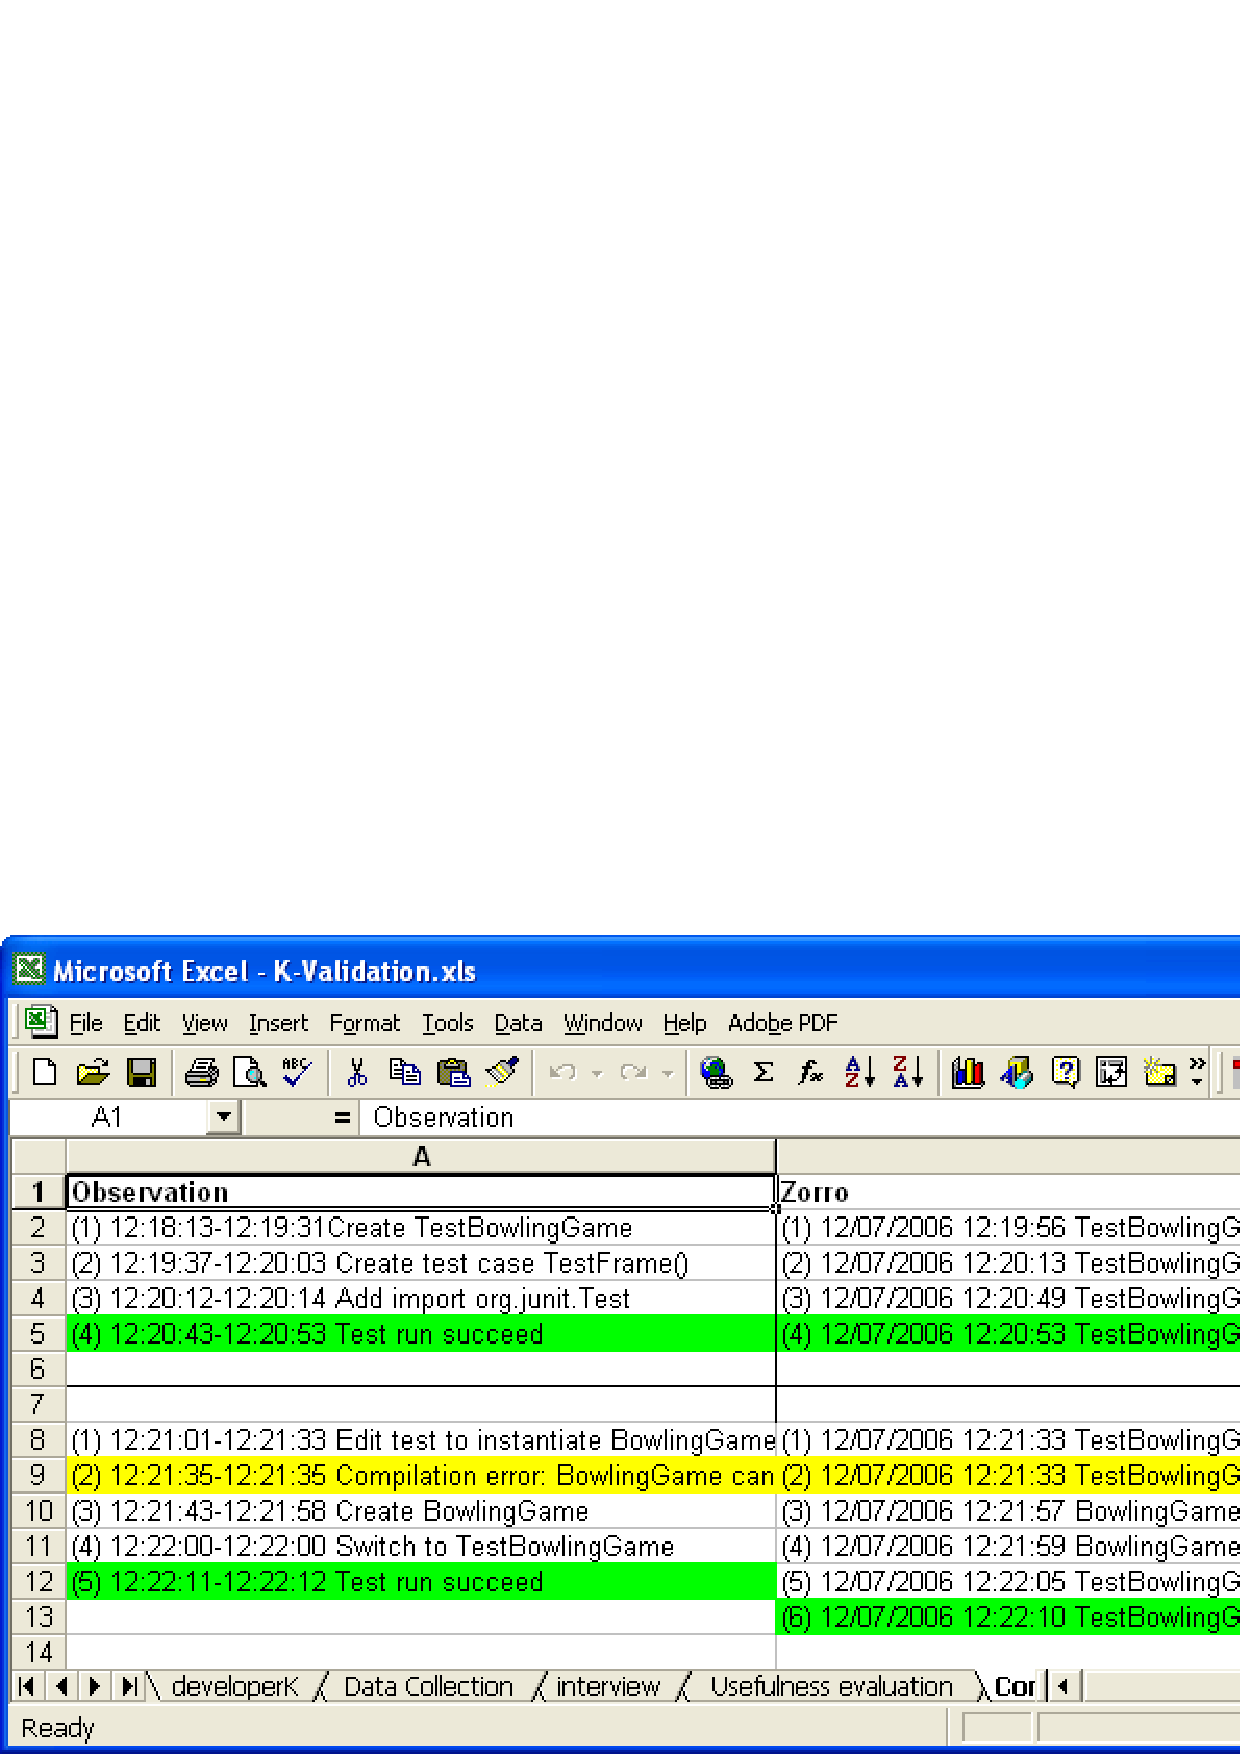
\includegraphics[width=1.0\textwidth]{figs/ZorroSensorDataValidation}
  \caption{Validation of Zorro's Development Activities}
  \label{fig:ZorroDataValidation}
\end{figure}

With side by side comparison (Figure \ref{fig:ZorroDataValidation}), I found two categories of situations that were responsible for Zorro's excessive data collection in the following. First, Zorro sometimes reported two or more activities while I only observed one development activity as what I described in the item of ``Kill two birds with one stone''. Second, though technically ESR should capture everything that happens in the Eclipse IDE, it did not in situations that were described in items of ``Invisible editing activities'' and ``Problems view of Eclipse could be hidden''. %Nearly 100\% of development behaviors I observed in ESR videos could be found in Zorro, but the relationship was not always one-to-one. Sometimes Zorro 

\begin{enumerate}
\item Kill two birds with one stone
  
When a developer changed statements that were associated with object components such as import, package declaration, attributes, method name, method return type, or method parameters, the Eclipse sensor collected two types of development activities: editing and refactoring. Similarly the Eclipse sensor would also collect both types of development activities when a developer used refactoring commands supplied in Eclipse. In both cases, Zorro doubled development activities. 

\item The problems view of Eclipse was hidden
  
In videos of participants `K', `M', and `T', the problems view of Eclipse was overlapped by other views for a while (see Figure \ref{fig:InvisibleEclipseProblemView}). I cannot observe compilation errors in this situation because Eclipse reports them in the problems view.  For instance, in Figure \ref{fig:InvisibleEclipseProblemView}, the JavaDoc view overlapped the problems view.  Since the title of the problems view was highlighted, it probably meant that there should have had compilation errors, but I could not tell it by watching the ESR video. 
  \begin{figure}[htbp]
    \centering
    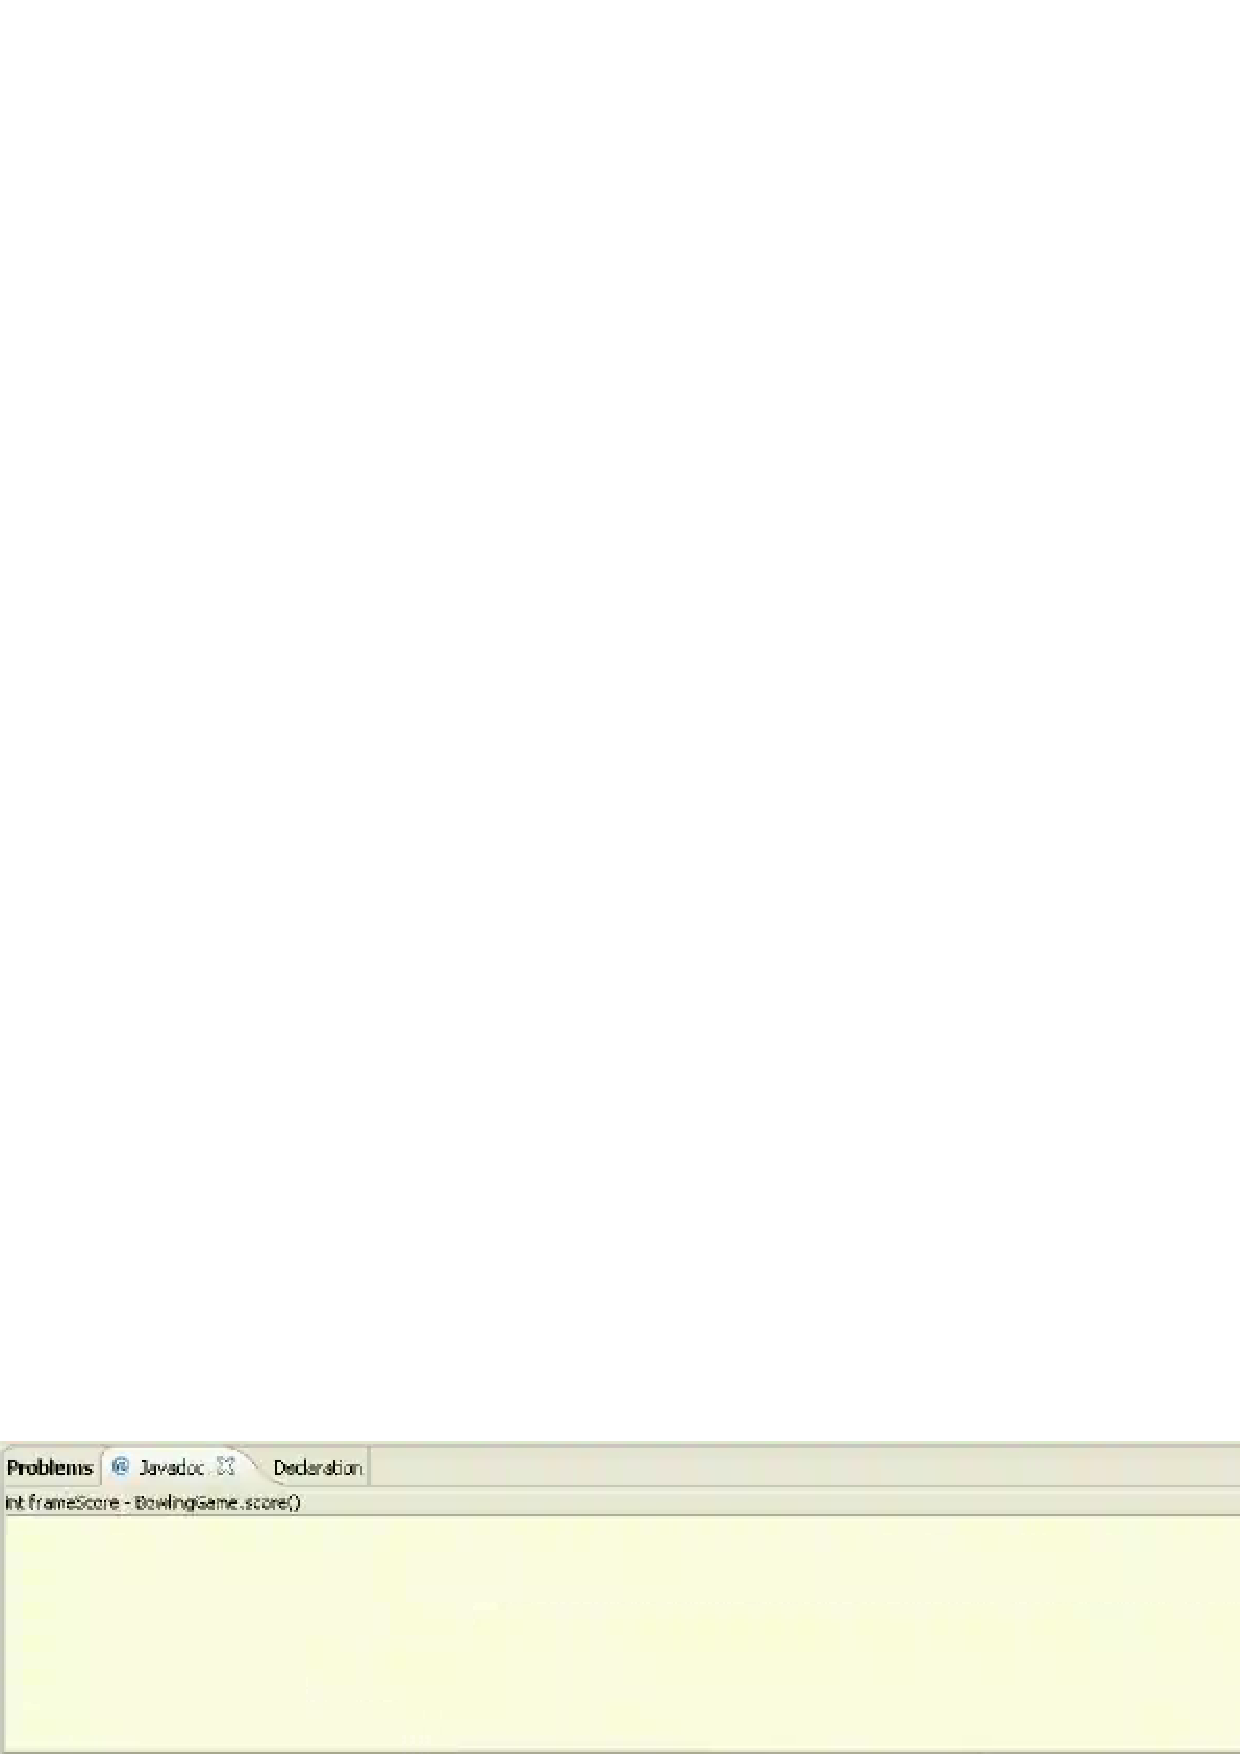
\includegraphics[width=0.8\textwidth]{figs/ESR-InvisibleProblemPane}
    \caption{Invisible Problems View in Eclipse}
    \label{fig:InvisibleEclipseProblemView}
  \end{figure}  

\item Invisible editing activities

A developer could input a few blank spaces while programming. Since ESR captured the screen of Eclipse, I would not be able to observe this kind of development activities because there is no visible changes. 

\end{enumerate}

The above three items can answer why Zorro collected more development activities than what I observed in recorded videos. However, there were also a few cases in which Zorro missed development activities (see items ``Quick editing'' and ``Quick buffer transition'').
\begin{enumerate}
 
\item Quick editing

The Eclipse sensor uses ``state change'' as the foundation to detect editing development activities. A timer thread in the sensor wakes up every 10 seconds to check the active buffer. If there are any changes made to the active buffer, the sensor will fire a ``state change'' event. Zorro reduces a series of consecutive ``state change'' events into an editing activity when processing development streams. This mechanism works well unless a developer edits a file for less than 10 seconds and then switches to another buffer. If so, the Eclipse sensor will miss an editing development activity.

\item Quick buffer transition
  
The Eclipse sensor collects ``buff trans'' activities by checking the active buffer.  A timer thread wakes up every 5 seconds to detect whether there is a buffer transition activity. Five-second is a small time period, but it is long enough for a developer to change the active buffers two or more times. If two or more consecutive buffer transition activities occur in less than 5 seconds, the Eclipse sensor might fail to capture some or all of them.
   
\end{enumerate}        

\subsubsection{Conclusion}
In this section, I summarized Zorro's data collection validation results (see Table \ref{tab:ActivityNumberSummary}). It turned out that Zorro collected more development activities per episode than I observed for every participant. Further investigation indicated that Zorro only missed a few development activities when participants quickly edited code or switched buffers. Also, Zorro collected development activities that were invisible in recorded videos. The analysis in this section indicates that there is partial supporting evidence for the research questions Q2a because Zorro can collect development activities more precisely than ESR, a recorder that can capture almost every development activity that occurs in the Eclipse IDE.  

\subsection{Validation of TDD Behaviors and TDD Compliance Inference}
\label{subsec:VideoObservationValidation}
Zorro recognizes TDD development through two steps (Chapter \ref{ch:Zorro}): (1) inferring development behaviors by matching development activities in episodes to a set of predefined development behaviors; (2) and then deducing TDD compliance using inferred episode behaviors. Thus, in this study, the validation analysis also had two steps: episode behavioral inference validation and TDD compliance inference validation, both of which were introduced in Section \ref{subsec:BehaviorComplianceValidation} for an individual participant. After validating Zorro for all participants, I summarized validation results in this section.

\subsubsection{Validation of Development Behavioral Inference}
\label{subsubsec:EpisodeBehavior}
For an individual participant I created a table similar as Table \ref{tab:BehaviorObservation} after validating Zorro's inference of his/her development behaviors. I then assigned the value 1 to an episode if the development behavior I observed in the video agrees with the development behavior Zorro inferred. In the end, I counted the number of 1's episodes and presented results in Table \ref{tab:EpisodeBehaviorAgreed} in which the last column is the percentage of 1's episodes to total episodes. This percentage could be an indicator of Zorro's development behavioral inference accuracy. 
\begin{table}[!ht]
\centering
  \caption{Video observation validation of development behaviors}
  \begin{tabular}{|l|r|r|r|}
  \hline
    ID & Episodes  & 1's Episodes & Percentage \\ \hline
    A       & 19   &  15   & 78.9\% \\ \hline  
    K       & 10   &   8   & 80.0\% \\ \hline
    L       &  8   &   7   & 87.5\% \\ \hline  
    N       &  9   &   4   & 44.4\% \\ \hline
    O       & 16   &  15   & 93.8\% \\ \hline
    P       & 18   &  12   & 66.7\% \\ \hline
    Q       & 21   &  11   & 52.4\% \\ \hline
    R       & 14   &  13   & 92.9\% \\ \hline
    S       &  9   &   2   & 22.2\% \\ \hline
    T       & 13   &   9   & 69.2\% \\ \hline
    Total   & 137  &  96   & 70.1\% \\ \hline
    \end{tabular}
  \label{tab:EpisodeBehaviorAgreed} 
\end{table}

In total, the participant observation analysis agreed that Zorro correctly inferred development behaviors in 96 episodes resulting in 70.1\% inference accuracy. But the inference accuracy is inconsistent from participant to participant. The lowest is 22.2\% and the highest is 93.8\% (Table \ref{tab:EpisodeBehaviorAgreed}). 

To address this inconsistency, one thing we can do is to study the impact of G2-DevBehavior by separating Table \ref{tab:EpisodeBehaviorAgreed} into two sub-tables: one for group G1 (Table \ref{tab:EpisodeBehaviorAgreedG1}), and the other one for group G2 (Table \ref{tab:EpisodeBehaviorAgreedG2}). 
\begin{table}[!ht]
\centering
  \caption{Video observation validation of development behaviors for G1}
  \begin{tabular}{|l|r|r|r|}
  \hline
    ID & Episodes  & 1's Episodes & Percent \\ \hline
    K       & 10   &   8   &  80.0\%  \\ \hline
    L       &  8   &   7   &  87.5\%  \\ \hline  
    O       & 16   &  15   &  93.8\%  \\ \hline
    R       & 14   &  13   &  92.9\%  \\ \hline
    Total   & 48   &  43   &  89.6\%  \\ \hline
    \end{tabular}
  \label{tab:EpisodeBehaviorAgreedG1} 
\end{table}
\begin{table}[!ht]
\centering
  \caption{Video observation validation of development behaviors for G2}
  \begin{tabular}{|l|r|r|r|r|}
  \hline
    ID & Episodes  & 1's Episodes & Percent & Episodes with G2-DevBehavior\\ \hline
    A       & 19   &  15   &  78.9\%  & 3  \\ \hline  
    N       &  9   &   4   &  44.4\%  & 3  \\ \hline
    P       & 18   &  12   &  66.7\%  & 4  \\ \hline
    Q       & 21   &  11   &  52.4\%  & 9  \\ \hline
    S       &  9   &   2   &  22.2\%  & 2  \\ \hline
    T       & 13   &   9   &  69.2\%  & 3  \\ \hline
    Total   & 89   &  53   &  59.6\%  & 24 \\ \hline
    \end{tabular}
  \label{tab:EpisodeBehaviorAgreedG2} 
\end{table}
Clearly, Zorro performed much better on inferring development behaviors for group G1 than for group G2. For G1, the average inference accuracy was 89.6\%, which is much higher than the average accuracy for G2. It indicates that G2-DevBehavior, which affected 24 out of 89 episodes, had a substantial impact on the accuracy of Zorro's inference of development behaviors. 

%In the best case, Zorro inferred 78.9\% of episode behaviors correctly for group G2 participants; on the contrary, even the lowest inference accuracy for group G1 participants is already 80.0\%. Of 89 episodes in Table \ref{tab:EpisodeBehaviorAgreedG2}, 24 were affected by the G2-DevBehavior. So it had great impacts on Zorro's development stream partition and episode behavior inference.

\subsubsection{Validation of TDD Compliance Inference}
Table \ref{tab:BehaviorObservation} lists not only development behaviors I observed but also TDD compliance for an individual participant. An episode is TDD compliant if its development behavior is either a portion of a TDD iteration such as refactoring or a complete TDD iteration. After observing TDD compliance for all participants, I summarized results in Table \ref{tab:TDDCompliantEpisodeNumber} for validation. 

%Zorro partitions a participant's development stream into episodes and infers the TDD compliance of those episodes. An episode is TDD compliant if its development behavior is either a portion of a TDD iteration, such as refactoring, or a complete TDD iteration. Beyond validating episode behavior inference, I also validated Zorro's TDD compliance inference. Table \ref{tab:TDDCompliantEpisodeNumber} lists the validation results. In the ``TDD Compliant Episodes'' columns, I include the number of TDD compliant episodes inferred by Zorro, the number of TDD compliant episodes I observed in the videos, and the difference between them for each participant. 
\begin{table}[!ht]
\centering
  \caption{Video observation validation of TDD compliance}
  \begin{tabular}{|l|r|r|r|r|}
  \hline
    &  &  \multicolumn{3}{c|}{TDD Compliant Episodes} \\ \cline{3-5}
    \raisebox{1.5ex}[0pt]{ID} & \raisebox{1.5ex}[0pt]{Episodes}  & 
     By Zorro &  By Video Analysis & Difference\\ \hline
    A       &  19   &  10    &  12  & -2  \\ \hline  
    K       &  10   &   9    &  10  & -1  \\ \hline
    L       &   8   &   7    &   7  &  0  \\ \hline  
    N       &   9   &   6    &   8  & -2  \\ \hline
    O       &  16   &  15    &  16  & -1  \\ \hline
    P       &  18   &  16    &  18  & -2  \\ \hline
    Q       &  21   &  21    &  21  &  0  \\ \hline
    R       &  14   &  13    &  14  & -1  \\ \hline
    S       &   9   &   3    &   9  & -6  \\ \hline
    T       &  13   &  13    &  13  &  0  \\ \hline
    Total   & 137   & 113    & 128  & -15 \\ \hline
    Mean    &      &        & 	& -1.5 \\ \hline
    Median  &      &        & 	& -1  \\ \hline
    STDEV   &      &        & 	& 1.78 \\ \hline
    \end{tabular}
  \label{tab:TDDCompliantEpisodeNumber} 
\end{table}
In Table \ref{tab:TDDCompliantEpisodeNumber}, the ``TDD Compliant Episodes'' column has numbers of TDD compliant episodes. It is divided into three sub-columns: ``By Zorro'', ``By Video Analysis'' and ``Difference''. With values in Table \ref{tab:TDDCompliantEpisodeNumber}, we can compute percentages of TDD compliant episodes in the following:
\begin{eqnarray}
%\[
   TDD(Zorro)\% & = & \frac{CompliantEpisodes(Zorro)}{TotalEpisodes} * 100 \nonumber \\
                & = & \frac{113}{137} * 100 \nonumber \\
                & = & 82.5, \nonumber \\ 
                            \nonumber \\
%\]
%\[
   TDD(Video Analysis)\% & = & 
                     \frac{CompliantEpisodes(VideoAnalysis)}{TotalEpisodes} * 100 \nonumber \\
                         & = & \frac{128}{137} * 100 \nonumber \\
                         & = & 93.4. \nonumber 
%\]
\end{eqnarray}

Using episode numbers as the measurement, Zorro is somewhat conservative on inferring TDD compliance compared to the participant observation analysis. The latter found that participants in this study complied to TDD in 93.4\% of episodes, while Zorro inferred that 82.5\% of episodes were TDD compliant. In Table \ref{tab:TDDCompliantEpisodeNumber}, I computed the episode number difference for all participants. The mean value is -1.5 and the standard deviation is 1.78, both of which are very small. %Thus, the participant observation analysis validation provides supporting evidence to the research question Q2b: \textit{Does Zorro�s inference of TDD behaviors agree with analyses based upon participant observation?}

However, the above evidence was not sufficient because the sample size was too small. Eleven  students participated in this study and I can only analyze data collected from 10 of them. In order to generalize research conclusions, it is necessary to include more participants. But the resource was limited in this study since the two software engineering classes only had 16 students (Section \ref{sec:ClassroomDesign}). 

%Fortunately, this limitation can be improved using the bootstrap resampling technique \cite{Resampling}. 

\begin{comment}
Resampling has many types and one of them is bootstrapping that can be used to estimate the precision of sample statistics \cite{Resampling} such as confidence interval and distribution of the sample mean. Bootstrap sampling is to sample randomly with replacement from a set of data points. In Figure \ref{fig:Bootstrap}, Dr. Teknomo introduced it using five balls and a basket to illustrate how it works. 
\begin{figure}[htbp]
  \centering
  \includegraphics[width=0.4\textwidth]{figs/BootstrapSampling}
  \caption{Randomly Sampling with Replacement \cite{BootstrapTutorial}}
  \label{fig:Bootstrap}
\end{figure}
Suppose that a sample contains 5 observations. We label them with 5 balls named `A', 'B', 'C', 'D', and 'E', and then put them into the basket. We randomly draw one ball from the basket, record its name, and then put it back into the basket. This is sampling with replacement with which we can increase sample size even though the available sample size is small. 

With bootstrapping, I raised sample size from 10 to 200 and computed descriptive statistic values (Table \ref{tab:BootstrapTDDPercent}). Note that the significant level was 0.05 (alpha value). 
\begin{table}
  \centering
  \caption{Descriptive Analysis of TDD\% with Bootstrapping}
  \begin{tabular}{|l|l|l|} \hline
                &  TDD\% (Zorro) & TDD\% (Video Analysis) \\ \hline
    Mean        &  80.4          & 93.9    \\ \hline
    Median      &  88.9          & 100.0   \\ \hline
    STDEV       &  21.3          & 11.4    \\ \hline
    Lower Bound &  63.8          & 85.3    \\ \hline 
    Upper Bound &  94.8          & 100.0   \\ \hline
  \end{tabular}
  \label{tab:BootstrapTDDPercent}  
\end{table}
According to Zorro's inference, the mean of participants' TDD compliance was 80.4\%. It indicates that Zorro can infer the compliance to TDD when it happens. Since participants did not comply to TDD all the time (93.9\%), Zorro's TDD compliance inference accuracy should be higher than 80.4\%. However, the standard deviation 21.3 was a little high and the confidence interval is a little wide ([63.8\%, 94.8\%]). 
\end{comment}

Next, I will discuss whether and how G2-DevBehavior affected Zorro's TDD inference by separating participants into groups G1 and G2. 

%However, this judgment is a bit premature because the mean and standard devision are not sufficient. A convincing conclusion must be accompanied by much stronger statistics analyses. In the next paragraph I will briefly introduce the goodness-of-fit of model to data, a statistics analysis method plausible for evaluating the fitness of Zorro's inference results to my video analysis results.

\begin{comment}
Since there are two sets of data, a temptation is to apply a parameter statistics test such as the t-test and f-test, or a nonparameter statistics test such as the chi-square test \cite{GoodnessOfFit,Anderson:86}, but none of them is appropriate for testing the goodness-of-fit. Fundamentally, statistics tests are meant to find evidence that the difference between the two or more sets of data is not caused by chance. In term of validating how accurately Zorro infers TDD, we are looking for some measures that can indicate how well Zorro is doing. Sadly, there are no formal standards with regard to the goodness-of-fit analysis method according to \cite{Schunn:05}. As a result, there are various methods and they are often used  incorrectly. In \cite{Schunn:05}, Schuun and Wallach recommend a combination of $r^2$ and RMSD (root mean squared  deviation) or RMSSD (root mean squared scaled deviation). $r^2$ is the square of Pearson correlation coefficient $r$ \cite{Anderson:86}. It measures how well relative trend magnitudes are captured \cite{Schunn:05}. That is, how well Zorro's inference predicates the video analysis. Note that $0\leq r^2 \geq1$. If $ r^2=1 $, Zorro's inference of TDD fits the video analysis perfectly. The $r^2$ alone is not sufficient for measuring goodness-of-fit because even a poor model can fit data very well in trend. It has to be combined with measures of deviation from exact location \cite{Schunn:05}. In my dissertation, I will use the root mean squared deviation (RMSD) \cite{Schunn:05} as the measure of deviation from exact location. Equation \ref{RMSD-Equation} explains how to compute the RMSD value.
\begin{equation} \label{RMSD-Equation}
  RMSD = \sqrt{MSD} = \sqrt{\frac{\sum^{n}_{i = 1}(m_{i} - d_{i})^2}{n}},
\end{equation}
where $m_{i}$ is the number of TDD compliant episodes inferred by Zorro for the $ith$ participant, $d_{i}$ is the number of TDD Compliant episodes I analyzed in the video for the same participant, and $n$ is the number of participants. 

Suppose that Zorro is the model of TDD compliance and my video analysis is the actual data that Zorro simulates, the $r^2$ value is 0.90 using the data in  Table \ref{tab:TDDCompliantEpisodeNumber}. It means that Zorro infers TDD compliance correctly 90\% of the time. It should be good enough to support that Zorro can infer TDD compliance correctly. Similarly, the RMSD value is 2.26 using the Equation \ref{RMSD-Equation}. Because the RMSD value changes when the scale changes, there is no such a standard that can tell how significant it is. But 2.26 is not a small number compared to the total number of episodes for each participant. As a conclusion, Zorro models the TDD compliance correctly with 90\% accuracy, but there is a tendency that it might overfit the video analysis because of the high RMSD value. 
\end{comment}

\begin{comment}

In order to get a sense of how the Zorro's inference results fit the video observation results, I will run the Chi-Square goodness-of-fit test. The goodness-of-fit test is to test whether a given distribution fits a set of data by comparing an observed frequency with the hypothesized distribution \cite{GoodnessOfFit,Anderson:86}. Letting $}p_{1}, p_{2}, ..., p_{10} $ denote the percentages of TDD compliant episodes for participants inferred by Zorro, the null hypothesis would be
\[
    H: p_{1} \neq p_{10},p_{2} \neq p_{20}, ..., p_{10} \neq p_{100}, 
\]
where \begin{math}p_{10},p_{20}, ..., p_{100} \end{math} are the percentages of TDD compliant episodes I observed in the process videos. If Zorro inferred TDD compliance accurately, we will reject the null hypothesis.

Let \begin{math}E_{i}\end{math} denote the expected number of TDD compliant episodes for the \textit{ith} participant and \begin{math}O_{i}\end{math} denote the number of TDD compliant episodes inferred by Zorro. The Chi-Square test is
\begin{equation} \label{ChiEquation}
  \chi^2 = \sum_{i=1}^{10}\frac{(O_{i}-E_{i})^2}{E_i}.
\end{equation}
Using the above equation we can get that the \begin{math}\chi^2\end{math} 
value is 5.28. The analysis power (p-value) of this test is is 0.81. 
It is great enough to reject the null hypothesis. Therefore, 
there are both arithmetic and statistic evidence that Zorro 
can infer TDD compliance according to the video observation 
analysis. Next, I will discuss whether the G2-DevBehavior has
any impact on Zorro's TDD compliance inference.
\end{comment}

\subsubsection{Discussion of G2-DevBehavior's Impact on TDD Compliance Inference}
Using G2-DevBehavior we can separate Table \ref{tab:TDDCompliantEpisodeNumber} into two sub-tables: one for group G1 (Table \ref{tab:TDDComplianceG1}) and the other one for group G2 (Table \ref{tab:TDDComplianceG2}). 

%In Section \ref{subsubsec:EpisodeBehavior}, we learned that G2-DevBehavior had had great impacts on Zorro's episode behavior inference. In order to investigate its impacts, I am going to separate the participants in Table \ref{tab:TDDCompliantEpisodeNumber}.  Table \ref{tab:TDDComplianceG1} lists the TDD compliance validation results using video observation analysis for group G1 participants, and Table \ref{tab:TDDComplianceG2} lists the validation results for group G2 participants.
\begin{table}[!ht]
\centering
  \caption{Validation of TDD Compliance Inference for Group G1}
  \begin{tabular}{|l|r|r|r|r|}
  \hline
    &  &  \multicolumn{3}{c|}{TDD Compliant Episodes} \\ \cline{3-5}
    \raisebox{1.5ex}[0pt]{ID} & \raisebox{1.5ex}[0pt]{Episodes}  & 
     By Zorro &  By Video Analysis & Difference \\ \hline
    K       & 10   &   9  & 10   & -1    \\ \hline
    L       &  8   &   7  &  7   &  0    \\ \hline  
    O       & 16   &  15  & 16   & -1    \\ \hline
    R       & 14   &  13  & 14   & -1    \\ \hline 
    Total   & 49   &  45  & 48	 & -3    \\ \hline 
    Mean &      &      &  & -0.75 \\ \hline
    Median  &      &      &  & -1    \\ \hline
    STDEV   &      &      &  & 0.5   \\ \hline
    \end{tabular}
  \label{tab:TDDComplianceG1} 
\end{table}
\begin{table}[!ht]
\centering
  \caption{Validation of TDD Compliance Inference for Group G2}
  \begin{tabular}{|l|r|r|r|r|r|}
  \hline
    &  &  \multicolumn{4}{c|}{TDD Compliant Episodes} \\ \cline{3-6}
    \raisebox{1.5ex}[0pt]{ID} & \raisebox{1.5ex}[0pt]{Episodes}  & 
     By Zorro &  By Video Analysis & Difference & G2-DevBehavior\\ \hline
    A       & 19 &  10   &  12  & -2   & 1 \\ \hline  
    N       &  9 &   6   &   8  & -2   & 1 \\ \hline
    P       & 18 &  16   &  18  & -2   & 1 \\ \hline
    Q       & 21 &  21   &  21  & 0    & 0 \\ \hline
    S       &  9 &   3   &   9  & -6   & 2 \\ \hline
    T       & 13 &  13   &  13  & 0    & 0 \\ \hline
    Total   & 89 &  69   &  81	& -12  & 5 \\ \hline 
    Mean    &    &       &      & -2   &   \\ \hline
    Median  &    &       &      & -2   &   \\ \hline
    STDEV   &    &       &      & 2.2  &   \\ \hline
  \end{tabular}
  \label{tab:TDDComplianceG2} 
\end{table}
There is noticeable difference between Table \ref{tab:TDDComplianceG1} and Table \ref{tab:TDDComplianceG2}. Using participant observation analysis results as the benchmark, Zorro inferred many fewer episodes as TDD compliant for group G2 than for group G1. Zorro's inference has a wide confidence interval because of the G2-DevBehavior. The standard deviation was 0.5 for group G1 in contrast to 2.2 for group G2.  

Next, I will discuss the inference errors that were unrelated to the G2-DevBehavior.

%In order to study how significant this difference is, I used bootstrapping again to increase sample sizes to 200 for both G1 and G2. 

%The mean value of  episode number differences for G1 is only -0.75 (see Table \ref{tab:TDDComplianceG1}), while the mean values for  G2 is -2 (see Table \ref{tab:TDDComplianceG2}). The G2-DevBehavior is responsible for the TDD compliance inference errors of 5 episodes.

\begin{comment}
Tables \ref{tab:BootstrapTDDPercentG1} and \ref{tab:BootstrapTDDPercentG2} listed the descriptive analysis results for G1 and G2 respectively. 
\begin{table}
  \caption{Descriptive Analysis of TDD Compliance with Bootstrapping for G1}
  \centering
  \begin{tabular}{|l|l|l|} \hline
                &  TDD\% (Zorro) & TDD\% (Video Analysis) \\ \hline
    Mean        &  91.1          & 96.7    \\ \hline
    Median      &  91.1          & 97.5    \\ \hline
    STDEV       &   1.1          &  2.5    \\ \hline
    Lower Bound &  89.1          & 92.5    \\ \hline 
    Upper Bound &  92.8          & 100.0   \\ \hline
  \end{tabular}
  \label{tab:BootstrapTDDPercentG1}  
\end{table}
\begin{table}
  \centering
  \caption{Descriptive Analysis of TDD Compliance with Bootstrapping for G2}
  \begin{tabular}{|l|l|l|} \hline
                &  TDD\% (Zorro) & TDD\% (Video Analysis) \\ \hline
    Mean        &  73.7          & 91.7    \\ \hline
    Median      &  74.7          & 92.6    \\ \hline
    STDEV       &  11.8          &  6.1    \\ \hline
    Lower Bound &  51.1          & 80.8    \\ \hline 
    Upper Bound &  93.3          & 100.0   \\ \hline
  \end{tabular}
  \label{tab:BootstrapTDDPercentG2}  
\end{table}
For G1, Zorro inferred TDD compliance accurately and consistently according to Table \ref{tab:BootstrapTDDPercentG1}. The confidence interval was very narrow ([89.1\%, 92.8\%]). In constrast, for G2, Zorro did not infer TDD compliance well. The mean of inference accuracy for G2 participants was 73.7\% and the confidence interval ([51.1\%, 93.3\%]) was very wide. So the G2-DevBehavior's impact on Zorro's TDD compliance inference was very significant. In other words, solving G2-DevBehavior has the potential to greatly improve Zorro's TDD compliance inference accuracy and consistency.  
\end{comment}

\begin{comment}
We can compute the goodness-of-fit measures for both of 
groups. Table \ref{tab:GoodnessOfFitMeasures} list the measures 
of G1 and G2 in conjunction with the measures of all participants.
\begin{table}[!ht]
\centering
  \caption{Measures of Goodness-of-fit}
  \begin{tabular}{lrr}
  \hline
             & $r^2$ & RMSD \\ \hline
    G1       &  0.99 & 0.88   \\ \hline
    G2       &  0.93 & 2.83   \\ \hline
    Overall  &  0.90 & 2.26   \\ \hline 
  \end{tabular} 
  \label{tab:GoodnessOfFitMeasures} 
\end{table}
In term of the $r^2$ measure, its value is 0.99 for G1 and 0.93 for G2, both of which exceed the overall value 0.90. Therefore, Zorro's inference is consistent within a group, and the inference results fit the video analysis results very well for both groups. But there is a big difference between two groups in term of $RMSD$, the measure of deviation from location. The $RMSD$ measure is 0.88 for G1 and 2.83 for G2. The previous value is much smaller than the overall value 2.26, while the latter is bigger than it. This could indicate that Zorro's inference is very off for participants in group G2, who conducted the ``G2DevBehavior''. Thus, the impact of ``G2DevBehavior'' is significant.
\end{comment}

%By separating participant into groups G1 and G2, we found that Zorro inferred TDD compliance perfectly for group G1, but the accuracy suddenly dropped to the unacceptable level for group G2 who ever conducted G2-DevBehavior. In other words, accommodating the G2-DevBehavior has the promise to greatly improve Zorro's TDD compliance inference capability. 

%We have shown that Zorro is conservative on inferring the episodes as TDD compliant episodes. The overall inference accuracy is acceptable according to the video observation validation although there are acceptance differences between group G1 and G2. In the next section, I am going to investigate why Zorro inferred less episodes as TDD compliant episode. 

\subsubsection{Discussion of Zorro's Inference Errors}
Out of 137 total episodes, Zorro inferred that 113 were TDD compliant, whereas the participant observation analysis validated that 128 were TDD compliant (see data in Table \ref{tab:TDDCompliantEpisodeNumber}). So the participant observation did not agree with Zorro's inference for 15 episodes. In Table \ref{tab:TDDComplianceG2}, we learned that the G2-DevBehavior 
caused the inference error for 5 episodes. In this section, I will investigate what happened to the remaining 10 episodes. 

It turned out that both Zorro's inference rules and participants' development behaviors played important roles for the inference errors.  To make it simple I will term all of these errors as ``Inference Error''. In Table \ref{tab:ZorroTDDComplianceInferenceError}, for each participant, I included episodes that are affected by both G2-DevBehavior and Inference-Error.
\begin{table}[!ht]
\centering
  \caption{Zorro's TDD Compliance Inference Error}
  \begin{tabular}{|l|r|r|r|r|r|r|}
  \hline
    &  &  \multicolumn{5}{c|}{TDD Compliant Episodes} \\ \cline{3-7}
    \raisebox{1.5ex}[0pt]{ID} & \raisebox{1.5ex}[0pt]{Episodes}  & 
     By Zorro &  By Video Analysis & Difference & G2-DevBehavior & Inference-Error\\ \hline
    A       &  19   &  10    &  12  & -2  & 1  & 1 \\ \hline  
    K       &  10   &   9    &  10  & -1  & 0  & 1 \\ \hline
    L       &   8   &   7    &   7  &  0  & 0  & 0 \\ \hline  
    N       &   9   &   6    &   8  & -2  & 1  & 1 \\ \hline
    O       &  16   &  15    &  16  & -1  & 0  & 1 \\ \hline
    P       &  18   &  16    &  18  & -2  & 1  & 1 \\ \hline
    Q       &  21   &  21    &  21  &  0  & 0  & 0 \\ \hline
    R       &  14   &  13    &  14  & -1  & 0  & 1 \\ \hline
    S       &   9   &   3    &   9  & -6  & 2  & 4 \\ \hline
    T       &  13   &  13    &  13  &  0  & 0  & 0 \\ \hline
    Total   & 137   & 113    & 128  & -15 & 5  & 10 \\ \hline
    \end{tabular}
  \label{tab:ZorroTDDComplianceInferenceError} 
\end{table}
We can see that each participant, except for participant `S', had at most one episode affected by G2-DevBehavior and one episode affected by Inference-Error. 

By carefully comparing development activities collected and behaviors inferred by Zorro (Figure \ref{fig:ZorroDataValidation}), I identified several causes for Inference-Error.
\begin{enumerate}
\item Additional production code editing before the next TDD episode

\textbf{Data Source}: 1 episode from participant `A' and 1 episode from participant `R'  \\
\textbf{Description}: After implementing a new feature, the TDD process typically requires a developer to refactor. Then the developer should rerun all the tests to make sure that the refactoring does not break anything. Should the developer rerun all the tests if the changes made to production code turn out to be very trivial? Strictly speaking, the answer for TDD is ``Yes''. Despite this, participants `A' and `R' refactored production code a small amount but opted not to run all tests. As a result, editing activities on production code fell into the following TDD episode. So the following episode began with production editing activity, which is inferred as a ``test-last'' episode. For example, the 9th episode from participant `A' was inferred as ``test-last'' because he refactored following code 
\begin{verbatim}
    int first;
    int second;
\end{verbatim}
to 
\begin{verbatim}
    int first = 0;
    int second = 0;
\end{verbatim}
but did not rerun all tests. 

\item No successful test invocations at the end

\textbf{Data Source}: 1 episode from participant `K' \\ 
\textbf{Description}: Successful test invocations are characteristic activities that mark the completion of a TDD iteration. An episode that does not end with successful test invocation is ``unknown'' to Zorro, and as a consequence, it is not TDD compliant. In this study, participant `K' did not finish the last user story; therefore, he ended with an ``unknown'' episode although he was doing TDD. %Of course, Zorro inferred it as not TDD compliant.

\item Insufficient Inference Rules

\textbf{Data Source}: 1 episode from participant `N', 1 episode from participant `O', and 1 episode from participant `P' \\ 
\textbf{Description}: The design of Zorro's TDD inference rules was rooted from the Red/Green/Refactor model in which tests should always have been created first. When test creations spread out in a TDD iteration, Zorro gets confused.  For example, in the 7th episode from participant `N', he added the test method ``TestGameScore()'' first, then implemented the functionality to compute the score of a bowling game, and then added assertion statements. So the test was created in two steps. As a result, this episode was wrongly inferred as ``test-last''. 

\item Unit tests were not properly structured

\textbf{Data Source}: 4 episodes from participant `S' \\ 
\textbf{Description}: Zorro recognizes the unit test class based upon the existence of test methods and assertion statements. A unit test could be wrongly recognized as production code, particularly at the beginning of a programming session when there are not any test methods or assertion statements. In this situation, Zorro infers the development behavior as ``test-last'', not ``test-first''. For example, test code in the first episode from participant `S' did not have any test method and assertion statement at the beginning. As a result, the first episode was inferred as ``test-last'' although participant `S' thought that he was doing TDD. In turn, due to the chain effect, following three refactoring episodes were also inferred as TDD noncompliant.

\end{enumerate}

\subsubsection{Conclusion}
In this section, using participant observation, I validated Zorro's inference of TDD development behaviors and TDD compliance. The validation indicates that Zorro inferred development behaviors with 70.1\% accuracy. Regarding TDD compliance, Zorro inferred that particpants in this study complied to TDD in 80.4\% of episodes, while participant observation indicates that 93.9\% of epsidoes were TDD compliant. The further discussion on G2-DevBehavior indicated that Zorro's inference accuracy and consistency would be improved if Zorro could correctly interpret G2-DevBehavior. 

In addition, to investigate causes for Zorro's inference errors, I compared development activities collected and behaviors inferred by Zorro to what I observed in ESR videos. Interestingly, most of the inference errors were caused by participants' nonstringent execution of TDD. Also, some of them were caused by insufficiently precise rules in Zorro.

%Moreover, I discussed the According to the video observation analysis, Zorro's inference results on TDD compliance are both arithmetically and statistically acceptable. The further discussions on G2-DevBehavior revealed that Zorro would infer the TDD compliance much more accurately if it accommodated the G2-DevBehavior. Next, I will address the supporting evidences to the research questions Q2a and Q2b (see Chapter \ref{ch:Research}).

\begin{itemize}
\item{\textbf{The culprit of G2-DevBehavior}}

I discovered the G2-DevBehavior in this study, the development behavior to invoke tests regardless of compilation errors. When it occurs, the test invocation may succeed, which leads to episode partitioning and development behavior inference errors. 

\item{\textbf{Research question Q2a: Does Zorro collect software development activities accurately enough for episode partition and TDD behavior inference?}}

This study provides evidence that Zorro collects a sufficient number of development activities accurately. Compared to participant observation using ESR, Zorro actually collected more development activities. A bug in the Eclipse sensor caused some data loss for one participant but I fixed it for the remaining 10 participants. The participant observation analysis validated that Zorro inferred development behaviors with 70.1\% accuracy and TDD compliance with more than 80.4\% accuracy. Both of these numbers would increase if Zorro could correctly interpret G2-DevBehavior. So the validation analysis in this section supports the research question Q2a.   

%Since students were lack of TDD development experiences, they were prone to make mistakes. According to the video observation analysis, G2-DevBehavior contributed to the inference errors.  Of 137 episodes, 24 were with either partition or inference errors in Table \ref{tab:EpisodeBehaviorAgreedG2}.  Despite this factor, only 15 of 137 episodes (see Table \ref{tab:TDDCompliantEpisodeNumber}) were inferred wrongly as noncompliant episodes according to the video observation analysis.

%The findings in the Section \ref{subsec:SensorDataValidation} indicate that there was partial evidence that Zorro collected enough development activities. In this section, we found that 24 episodes were partitioned wrongly and with inference errors, but the Zorro's inference accuracy was acceptable, compared to the video observation analysis. Therefore, there is supporting evidence to the research question Q2a.

\item{\textbf{Research question Q2b: Does Zorro's inference of TDD behaviors agree with analyses based upon participant observation?}}

According to participant observation, Zorro infers development behaviors correctly for 70.1\% of episodes. It infers that 80.4\% of episodes were TDD compliant while the particpant observation validated that 93.9\% of episodes were TDD compliant. 
%With 5\% significance level, the confidence interval of Zorro's TDD compliance inference was [63.8\%, 94.8\%]. The inference accuracy was acceptable but the variation was a bit large. 
Further discussion indicates that Zorro can perform better if there were not G2-DevBehavior, and only 3 out of 128 episodes have inference errors. All these conclusions provided supporting evidence to the research question Q2b. 

%Participants in this study conducted 137 episodes, of which 113 were TDD compliant according to Zorro and 128 were TDD compliant according to participant observation (see Table \ref{tab:TDDCompliantEpisodeNumber}). 

%Consequently, 15 episodes were with inference error, which resulted in 10.9\% of errors. With regard to episode behavior inference, Zorro's inference accuracy is 68.8\% (see Table \ref{tab:EpisodeBehaviorAgreed}). The goodness-of-fit statistics analysis in this section also demonstrated that Zorro's TDD compliance inference fit the video observation analysis very well. These conclusions provide supporting evidence to the research question Q2b.
\end{itemize}

\subsection{Cross-validation of Zorro using participant comments}
\label{subsec:ParticipantCommentAnalysis}
In the previous section, we have shown that participant observation agreed with Zorro's inference on development behaviors and TDD compliance. In this section, I will analyze participants' comments to cross-validate the research conclusions we have drawn above. 

%The participants used web interface to comment whether they were conforming to TDD and what development behaviors they conducted. The purpose of collecting the participants' comments is to cross-validate Zorro's TDD inference, in addition to the video observation validation. 

In Section \ref{subsec:ParticipantValidation}, I demonstrated how I conducted cross-validation analysis for one participant. Following the same method described in Section \ref{subsec:ParticipantValidation}, I analyzed all participants' comments and described validation results in the following. 

%In this section, I will put Zorro's TDD inference results, the video observation results, and participant comments together for the cross-validation. Table \ref{tab:ParticipantTDDBehavior} is an example comparing three of them for one participant. I will cross-validate Zorro's inference on TDD compliance first, and then focus on its episode behavior inference cross-validation. 

\subsubsection{Cross-validation of TDD Compliance Inference}
Table \ref{tab:ComparisonOfMethods} is a summary of cross-validation results for all episodes produced by participants in this study. An episode could be ``compliant'', ``noncompliant'', or ``don't know''. %The ``don't know'' episodes Note that only the participants ever commented some episodes as ``Don't know'' episodes in this study. 
\begin{table}[!ht]
\centering
  \caption{TDD Compliance Comparison}
  \begin{tabular}{|l|r|r|r|}
  \hline
    \backslashbox[35mm]{Method}{Episodes} & Compliant & Noncompliant & Don't know\\ \hline
    Zorro                                 &  110	& 27 & \\ \hline
    Video Analysis                        &  128	& 9  &  \\ \hline  
    Participant Comment                   &  111  & 11 & 15 \\ \hline
    \end{tabular}
  \label{tab:ComparisonOfMethods} 
\end{table}
Interestingly, based upon numbers in Table \ref{tab:ComparisonOfMethods}, participant comments on TDD compliance were much closer to Zorro's inference results than to participant observation analysis results. Participants commented that 111 episodes were TDD compliant, which is just 1 episode different from what Zorro inferred. %In contrast, the video analysis concluded that 128 episodes were TDD compliant. 

There are two possible explanations to this phenomenon. One explanation is that Zorro was really good at inferring TDD compliance. The other explanation is that participants simply went along with Zorro's perspective on their behaviors due to lack of experience with TDD. After reviewing Zorro's reasoning process and inference results, participants commented on their development behaviors. Therefore, in order to improve validity of participants' comments, I explained to them that their comments would help to improve Zorro's inference and encouraged them to read aloud while commenting. Also, I used a digital voice recorder to record their verbal comments. 

%Therefore, in order to use the participant comments wisely, I will compare them with both Zorro's inference results and my video observation analysis results. 

I listed detailed cross-validation results for all participants in Table \ref{tab:ComplianceParticipantValidation}. 
% Both the compliant and noncompliant episodes are from the three data sources: Zorro, video analysis, and participant comment. The ``don't know'' episodes are from participant comments only.
\begin{sidewaystable}[htbp]
  \centering
\begin{tabular}{|r|r|rrr|rrr|r|} \hline
  &  &  \multicolumn{3}{c|}{Compliant Episodes} 
     &  \multicolumn{3}{c|}{Noncompliant Episodes} & Don't know\\\cline{3-9}
  \raisebox{1.5ex}[0pt]{ID} & \raisebox{1.5ex}[0pt]{Episode} & 
   Zorro & Video Analysis  & Participant Comment &  Zorro & Video Analysis  & Participant Comment & Participant Comment\\ \hline
   A & 19 & 10 & 12 &  9 & 9 & 7 & 7 & 3 \\ \hline
   K & 10 & 9  & 10 &  9 & 1 & 0 & 0 & 1 \\ \hline
   L & 8  &  7 & 7  &  7 & 1 & 1 & 1 & 0 \\ \hline
   N & 9  &  6 & 8  &  7 & 3 & 1 & 0 & 2 \\ \hline
   O & 16 & 15 & 16 & 16 & 1 & 0 & 0 & 0 \\ \hline
   P & 18 & 16 & 18 & 18 & 2 & 0 & 0 & 0 \\ \hline
   Q & 21 & 19 & 21 & 17 & 2 & 0 & 0 & 4 \\ \hline
   R & 14 & 13 & 14 & 12 & 1 & 0 & 0 & 2 \\ \hline
   S & 9  &  3 &  9 &  7 & 6 & 0 & 2 & 0 \\ \hline
   T & 13 & 12 & 13 &  9 & 1 & 0 & 1 & 3 \\ \hline
   Total  & 137 & 110 &  128 &  111 &  27 & 9 & 11 & 15 \\ \hline
\end{tabular}  
  \caption{Participant Comments on TDD Compliance}
  \label{tab:ComplianceParticipantValidation} 
\end{sidewaystable}
Zorro inferred that 110 of 137 episodes were compliant and 27 were noncompliant. In contrast, the participant observation analysis validated that 128 were compliant and only 9 were noncompliant. Finally, participants commented that 111 were compliant, 11 were noncompliant, and 15 were neither of them. Most of the time, participants agreed that Zorro inferred their TDD compliance very well. When they were not sure to the TDD compliance of an episode, they declared it as ``Don't know''. Fifteen episodes are in this category. 

%The results were similar rather than different. To test how close the results are, we can compute the goodness-of-fit measures as what we have done in Section \ref{subsec:VideoObservationValidation}. Note that the ANOVA statistic test (Analysis of Variance) is not applicable at here due to the nature of my data analysis. In addition to this, TDD is the only treatment and we do not have any pretests to compare with. 

%First, let's use the participant comments as the additional data to cross-validate Zorro's TDD compliance inference. Since it is another kind of validation on Zorro's compliance inference, we can use the same notations as in Section \ref{subsec:VideoObservationValidation}.But $d_{i}$ denotes the number of TDD compliant episodes commented by the $ith$ participant. With Equation \ref{RMSD-Equation}, the $RMSD$ measure is 1.92. The $r^2$ measure is 0.83.  So Zorro's inference on TDD compliance is close to participants comments in both the trend and the deviation of location. 

%Now that the cross-validation strengthens the conclusion made on Zorro's TDD compliance inference in Section \ref{subsec:VideoObservationValidation}, we can readdress the G2-DevBehavior using the participant comments.

\begin{comment}
Let \begin{math}O_{i}\end{math} denote the number of TDD 
compliant episodes inferred by Zorro and
\begin{math}E_{i}\end{math} denote the number of TDD compliant
episodes commented by participants, for the \begin{math}ith\end{math}
participant. Using the Equation \ref{ChiEquation}, we would get that
the  and analysis power is
0.90. Certainly, this analysis power is high enough and we can say
that the participants strongly agree with Zorro's TDD inference.

Second, let's use the participant comments to verify the video observation analysis results. Let $m'_{i}$ denote the number of compliant episodes observed in the video of the $ith$ participant. We can modify the Equation \ref{RMSD-Equation} to  
\begin{equation} \label{RMSD-VerifyEquation}
RMSD = \sqrt{MSD} = \sqrt{\frac{\sum^{n}_{i = 1}(m'_{i} - d_{i})^2}{n}}.
\end{equation}
Using this modified equation, the $RMSD$ measure is 2.26. In addition, the $r^2$ measure is 0.88. So my video analysis is a fit model for participant comments, and the deviation of location is just as big as the same measure for video analysis validation computed in the Section \ref{subsec:VideoObservationValidation}. In others words, the video observation analysis method is dependable in validating Zorro's TDD compliance inference according to participant comments.
\end{comment}

\begin{comment}
observed by me using the video analysis and
\begin{math}E_{i}\end{math} denote the number of TDD compliant
episodes commented by the participants. We can modify the original
Chi-Square Equation \ref{ChiEquation} into
\begin{equation} \label{ChiVerifyEquation}
  \chi^2 = \sum_{i=1}^{10}\frac{(O'_{i}-E_{i})^2}{E_{i}}.
\end{equation}
Using this equation, the \begin{math}\chi^2\end{math} value is 4.88 and the analysis power is 0.84. Thus, we can not distinguish the differences between the participant comments and video analysis statistically with the chi-square test. In another word, there is supporting evidence that the video analysis method is not biased in this study.
\end{comment}

\subsubsection{Discussion of G2-DevBehavior}
\begin{comment}
When observing the development behaviors using the recorded ESR videos, I analyzed the TDD behaviors. The participants commented their development behaviors by recalling what they have done and referring to the collected development activities. Since both the participants and I were able to correct the G2-DevBehavior on the fly, it would be reasonable to assume that the G2-DevBehavior will have similar impacts on the video analysis and participant comment methods. 
\end{comment}

I broke Table \ref{tab:ComplianceParticipantValidation} into Table \ref{tab:ComplianceParticipantValidationG1} and Table \ref{tab:ComplianceParticipantValidationG2} by separating participants according to G2-DevBehavior.
\begin{table}[!ht] 
  \centering
  \caption{Group G1's comments on TDD Compliance}
\begin{tabular}{|r|r|rrr|rrr|} \hline
  &  &  \multicolumn{3}{c|}{Compliant} & \multicolumn{3}{c|}{Noncompliant} \\\cline{3-8}
  \raisebox{1.5ex}[0pt]{ID} & \raisebox{1.5ex}[0pt]{Episode} & 
   Zorro & Video Analysis  & Participant &  Zorro & Video Analysis  & Participant \\ \hline
  K & 10 &  9 & 10 &  9 &  1 & 0 & 0 \\ \hline
  L &  8 &  7 &  7 &  7 &  1 & 1 & 1 \\ \hline
  O & 16 & 15 & 16 & 16 &  1 & 0 & 0 \\ \hline
  R & 14 & 13 & 14 & 12 &  1 & 0 & 0 \\ \hline
  Total & 48 &  44 & 47 & 44 & 4 & 1 & 1 \\ \hline
  \end{tabular}  
  \label{tab:ComplianceParticipantValidationG1} 
\end{table}
\begin{table}[!ht] 
  \centering
  \caption{Group G2's comments on TDD Compliance}
\begin{tabular}{|r|r|rrr|rrr|} \hline
  &  &  \multicolumn{3}{c|}{Compliant} & \multicolumn{3}{c|}{Noncompliant} \\\cline{3-8}
  \raisebox{1.5ex}[0pt]{ID} & \raisebox{1.5ex}[0pt]{Episode} & 
   Zorro & Video Analysis  & Participant &  Zorro & Video Analysis  & Participant \\ \hline
 A & 19 &  10 & 12 &  9 & 9 & 7 & 7 \\ \hline
 N &  9 &   6 &  8 &  7 & 3 & 1 & 0 \\ \hline
 P &  18 & 16 & 18 & 18 & 2 & 0 & 0 \\ \hline
 Q &  21 & 19 & 21 & 17 & 2 & 0 & 0 \\ \hline
 S &   9 &  3 &  9 &  7 & 6 & 0 & 2 \\ \hline
 T &  13 & 12 & 13 & 9 &  1 & 0 & 1 \\ \hline
 Total & 89 & 66 & 81 & 67 & 23 & 8 & 10 \\ \hline
  \end{tabular}  
  \label{tab:ComplianceParticipantValidationG2} 
\end{table}
Participants in group G1 commented that Zorro almost perfectly inferred their TDD compliance (Table \ref{tab:ComplianceParticipantValidationG1}). It also showed that the participant observation analysis was not biased because these two analyses reached the same conclusion. Because of G2-DevBehavior, participants in group G2 did not completely agree with what Zorro inferred about their compliance to TDD, but the difference was not big (Table \ref{tab:ComplianceParticipantValidationG2}).

%In Section \ref{subsec:VideoObservationValidation}, we have proved that the G2-DevBehavior affected Zorro's TDD compliance inference using the video observation analysis. But its impact is not obvious based on the data in Table \ref{tab:ComplianceParticipantValidationG2}. Zorro  inferred that the number of TDD compliant episodes is 66, which is just one episode off to what participants commented. Therefore, it is necessary to test the goodness of fit for group G2. Using the Equation \ref{RMSD-VerifyEquation}, the $RMSD$ measure is 2.41. In addition, the $r^2$ measure is 0.81. They indicate that the fit between Zorro's inference and participant comments for G2 participants is poor. In other words, the participants in group G2 somewhat disagreed with Zorro on their compliance of TDD. In fact, they did acknowledge that Zorro inferred some of their development behaviors incorrectly due to their G2-DevBehaviors. 

\begin{comment}
Let \begin{math}O'_{i}\end{math} denote the number of compliant episodes observed by the video analysis and \begin{math}E_{i}\end{math} denote the number of TDD compliant episodes commented by participants. Using the equation  
\[
\chi^2 = \sum_{i=1}^{4}\frac{(O'_{i}-E_{i})^2}{E_{i}}
\]
on group G1, I got that the \begin{math}\chi^2\end{math} is 0.44 and the analysis power is 0.93. Using the equation
\[
\chi^2 = \sum_{i=1}^{6}\frac{(O'_{i}-E_{i})^2}{E_{i}}
\]
on group G2, I got that the \begin{math}\chi^2\end{math} is 4.43 and the analysis power is only 0.49. Surprisingly, the analysis power for group G2 is too weak to reject the null hypothesis. That is to say, if the participants commented the TDD compliance correctly, the video analysis would only get the same results in 49\% of chance. This is contradict to the assumption I just made at the beginning of this analysis. Thus, we need further investigation to find the causes.

After looking at the data in Table \ref{tab:ComplianceParticipantValidationG1} and Table \ref{tab:ComplianceParticipantValidationG2} carefully, you would find that the episode numbers from the video analysis and participant comments are not equal. In \ref{tab:ComplianceParticipantValidationG1}, the video analysis observed that 47 episodes were compliant and 1 episode was noncompliant. The sum of the two numbers is 48. In the same table, the participant commented that 44 episodes were compliant and 1 episode was noncompliant. The sum of the two numbers is only 45. 45 does not equal to 48 and 3 episodes were missed. The reason was that the participants commented the other 3 episodes as ``don't know''. In contrast, the participants in group G2 commented 11 episodes as ``don't know''. So the G2-DevBehavior could restrain the participants to comment their TDD compliance correctly.
\end{comment}

\subsubsection{Cross-validation of Episode Behavior Inference}
\label{subsec:ParticipantEpisodeBehavior}
Participants used the web page illustrated in Figure \ref{fig:EpisodeFeedback} to give their feedback after reviewing their development activities and remembering what they have done in an episode. Meanwhile, in order to get as much feedback as possible, I also recorded their verbal comments.

Participants commented on their episode behaviors by selecting from a set of development behaviors including ``adding new functionality'', ``adding test'', and ``just running tests'' etc. Therefore, in order to compare their comments with episode behaviors inferred by Zorro and that I observed in recorded videos, it is necessary to code their comments and build a mapping schema to connect them. Table \ref{tab:ParticipantCommentMapping} defines a mapping schema I used in this data analysis. 
\begin{table}[!ht] 
  \centering
  \caption{Mapping schema from participant's comment to Zorro/Video Analysis inference}
\begin{tabular}{|l|l|l|} \hline
  Participant Comments &  Relation & Zorro/Video Analysis \\ \hline
  adding new functionality + adding test + [more] + TDD & \(\equiv\) & test-first \\ \hline
  adding new functionality + adding test + [more] + \(\sim\)TDD & \(\equiv\) & test-last \\ \hline
  adding new functionality + [more] + TDD  & \(\equiv\) & test-first \\ \hline
  adding new functionality + [more] + \(\sim\)TDD & \(\equiv\) & production \\ \hline
  adding test + [just running tests] & \(\equiv\)  & test-addition \\ \hline
  adding test + [just running tests] + TDD & \(\equiv\) & test-first \\ \hline
  refactoring + [just running tests] & \(\equiv\) & refactoring \\ \hline
  just running tests & \(\equiv\) &  regression \\ \hline
  no comment & ? & anything \\ \hline
  other      & \(\neq\) & anything \\ \hline
  \end{tabular}  
  \label{tab:ParticipantCommentMapping} 
\end{table}
In the participant comments column, '+' means combination of development behaviors, a development behavior is optional if it is embraced by a pair of closed brackets, '\(\sim\)' sign stands for negation, and ``[more]'' matches any development behavior. In the relation column, '\(\equiv\)' stands for the equivalent relationship, '\(\neq\)' stands for the nonequivalent relationship, and the question mark '?' stands for the unsure relationship.
 
Using this mapping schema, I compared development behaviors indicated by participant comments to development behaviors inferred by Zorro. I marked an episode as ``agreed'' if I can map the participant's comment to the development behavior inferred by Zorro, ``disagreed'' if the two are not equivalent using the schema in Table \ref{tab:ParticipantCommentMapping}, or ``unsure'' if the participant did not comment or no mapping exists. Comparison results are available in Table \ref{tab:ParticipantBehaviorValidation}.  In addition, I also appended comparison results between participant observation and Zorro in the same table.
\begin{table}[!ht] 
  \centering
  \caption{Participant's Validation of Episode Behaviors}
\begin{tabular}{|r|r|rrr|rr|} \hline
  &  &  \multicolumn{3}{c|}{Participant v.s. Zorro} & 
        \multicolumn{2}{c|}{Video Analysis v.s. Zorro} \\\cline{3-7}
  \raisebox{1.5ex}[0pt]{ID} & \raisebox{1.5ex}[0pt]{Episode} & 
   Agreed & Disagreed  & Unsure &  Agreed & Disagreed  \\ \hline
  A & 19 & 12 & 5 & 2 & 15 & 4 \\ \hline
  K & 10 &  8 & 2 & 0 &  8 & 2 \\ \hline
  L &  8 &  6 & 2 & 0 &  7 & 1 \\ \hline
  N &  9 &  6 & 2 & 1 &  4 & 5 \\ \hline
  O & 16 & 14 & 2 & 0 & 15 & 1 \\ \hline
  P & 18 & 14 & 4 & 0 & 11 & 7 \\ \hline
  Q & 21 & 12 & 5 & 4 & 11 & 10 \\ \hline
  R & 14 & 12 & 1 & 1 & 13 & 1 \\ \hline
  S &  9 &  6 & 3 & 0 &  2 & 7 \\ \hline
  T & 13 & 10 & 2 & 1 &  9 & 4 \\ \hline
  Total & 137 & 100 & 28 & 9 & 95 & 42 \\ \hline
  \end{tabular}  
  \label{tab:ParticipantBehaviorValidation}
\end{table}
This table makes it clear that the participant comment analysis yielded very close findings to the participant observation analysis. With regard to agreed episodes, one is 100 and the other is 95. Numbers of disagreed episodes are also very close. So, on the episode level, participant comments agree with participant observation results. This provides strong evidence that the video analysis method is not biased in this study. 

Regarding G2-DevBehavior, participants in group G2 were more likely to disagree with Zorro's inference of their development behaviors. For example, developer `N' noticed that ``one episode goes into two because I ran the test before adding [the production code].'' Developer `P' commented that ``[when there is compilation error], JUnit does tell test failures if the method is not found. It is a JUnit problem not Eclipse.'' Participant `Q' also pointed out that one of his episodes was not partitioned correctly. Participant `T' even brought up the G2-DevBehavior problem before validating Zorro. 

\subsubsection{Conclusion}
In this section, I analyzed participant comments to cross-validate Zorro's inference on TDD compliance and development behaviors. 

With regard to TDD compliance, participants agreed with Zorro's inference results and the participant observation analysis results (see Table \ref{tab:ComparisonOfMethods}). Thus, the cross-validation provides evidence that participant observation is a viable method for validating Zorro. By separating participants into groups G1 and G2, we found that participants almost completely agreed with Zorro's inference results and participant observation analysis results for participants in group G1. 

%The further goodness of fit tests provided strong evidence for this conclusion. The $r^2$ measure between Zorro's inference and participant comments is 0.83, with $RMSD$ measure 1.92. It is strong enough to provide supporting evidence for the research question Q2c (see Chapter \ref{ch:Research}). The $r^2$ measure between the video analysis and participant comments is 0.88, which supports the statement that the video analysis is not biased for Zorro validation. This can strengthen the conclusion we have made in Section \ref{subsec:VideoObservationValidation} for the research question Q2b.

Though participant comments provided strong evidence to research question Q2c, we must be cautious because the conclusion could be influenced by a caveat problem -- the participant's knowledge of Zorro's inference. I advised participants use Zorro's inference results as reference only and encourage them to read aloud to give us feedback for Zorro improvement. The cross-validation analysis in this section provides some evidence that participants were able to comment independently. They commented 15 episodes as ``don't know'' to express their disagreements with Zorro's inference.

With regard to episode behaviors, I built a development behavior mapping schema to map participant comments to development behaviors Zorro inferred and to those that I observed in recorded videos. According to Table \ref{tab:ParticipantBehaviorValidation}, participants agreed that Zorro inferred development behaviors in 73.0\% (100 of 137) of episodes correctly. In comparison, the participant observation analysis validated that Zorro inferred development behaviors in 69.3\% (95 of 137) of episodes correctly. Both validation analyses concluded that Zorro is capable of inferring development behaviors, but there is still room for improvements.

\subsection{Participant interview analysis}
\label{subsec:ParticipantInterviewAnalysis}
Before this study, the instructor of the software engineering classes introduced TDD to students after they finished the semester-long course projects. Unit testing was a required practice in their course projects. The students also practiced what they had learned in the TDD lecture using 
the Roman numeral conversion problem (see Appendix \ref{app:UserStoriesRomanNumeral}).

Following the interview guideline in Appendix \ref{app:CaseStudyInterviewGuide}, I interviewed participants on unit testing and TDD at the end of this study. Then I processed the interview script using the coding research method \cite{Creswell:03,GroundedTheory} to categorize the participants.

\subsubsection{Unit Testing Survey}
Among the participants, only one has used unit testing for a long time at work, one had practiced unit testing for a while, and the others had just started to learn unit testing since the beginning of the software engineering classes. Since most participants were new to unit testing, I decided not to differentiate them based on unit testing experience in the coding process.

The participants unanimously agreed that unit testing is good for software development, but they had a diversity of opinions on how helpful unit testing is. However, some of them pointed that unit testing was hard sometimes, especially when they wanted to achieve 100\% test coverage. 

In the open coding stage, I wrote down the values of properties including unit testing assessment, experience, testing behavior, testing effort and test coverage. I categorized participants based on these properties. Using coding and memoing methods, I categorized the participants and listed the core categories in Table \ref{tab:UnitTestingCategory} based upon the property values.
\begin{table}[htbp]
\centering
  \caption{Participant Categories on Unit Testing}\label{tab:UnitTestingCategory}  
  \begin{tabular}{|l|p{5cm}|l|}
  \hline
    Category &  Description & Participant \\ \hline
    Good-but-Small-Effort & Test is good for quality but I do not 
                            write test often and I have excuses. & A, L, O, P, R, S, and T \\ \hline
    Must-and-Test-Last & All code must have unit test. The work flow is 
                         design, think, code and test. & K \\ \hline
    VeryGood-and-Much-Effort & Test is very good and I spent quite some effort on it & 
                               N and Q \\ \hline
    \end{tabular}
\end{table}

The majority of the students acknowledged that unit testing is good for improving software quality but they did not devote enough effort on it. 

\subsubsection{TDD Survey}
TDD is very different from unit testing. It not only reverses the order of production and test developments, but also advocates unit tests as the driving force for software design. I coded the interview data using properties including TDD's impacts on unit testing and software quality, and how hard it is to develop software in TDD. Table \ref{tab:TDDPerceptionCategory} lists the core categories.
\begin{table}[htbp]
\centering
  \caption{Participant Categories on Perception of TDD}\label{tab:TDDPerceptionCategory}  
  \begin{tabular}{|l|p{5cm}|l|}
  \hline
    Category &  Description & Participant \\ \hline
    Negative & Messy design. Straight TDD is weird. & K and S\\ \hline
    No-Change & No guarantee for quality. May take longer such that yields better quality. 
                            & A and L \\ \hline 
    Positive-With-Condition & More time on testing and better testing. Hard
                              if there is no good to-do list. Helpful when from scratch up.
                              Eclipse discourages TDD because of compilation error warning. 
                              & N, O, P, Q, R, and T \\ \hline
    \end{tabular}
\end{table}

\begin{comment}
TDD sometimes has negative or zero effect on developers' software development. There is no guarantee for high quality and good design with TDD. Severn participants quoted that TDD may work well under certain circumstances. Good To-Do list is necessary for carrying TDD project, and TDD can benefit a project if it is from scratch up. Eclipse, the IDE used in this study, discouraged TDD practice because it warned developers when the tested code did not exist yet.
\end{comment}

A common misunderstanding of the participants is that developers should create the complete To-Do list prior to implementation, which is not true for TDD. Instead, developers should dynamically maintain the To-Do list by themselves. It is reasonable that they had this impression given the experiment settings of this study. I provided the user stories to help participants develop solutions for the bowling game problem (Appendix \ref{app:UserStoriesBSK}) without spending a lot of time to ensure that they understood the bowling game scoring methods. This is a trade-off we had to take because previous studies found that it could take participants up to 48 hours to accomplish the same programming problem \cite{Erdogmus:05}. Based on lessons learned from others, providing the user stories that are easy to understand is necessary for this study's experimental design, which required a reasonable number of TDD iterations to be completed within 90 minutes. Given that my research interest is on validating Zorro's automated inference, providing user stories is acceptable. In the interview, I explained to participants that they should dynamically maintain the To-Do list by themselves in real situations.

\subsubsection{TDD Acceptance Survey}
Last, I asked participants how they would respond if their project managers required everybody to use TDD. Two developers would be against the use of TDD in daily software development. Three developers would accept it if good design documentation and To-Do lists are in place. The remaining five participants would be very willing to use TDD. Table \ref{tab:TDDAcceptanceCategory} listed the participant categories.
\begin{table}[htbp]
\centering
  \caption{Participant Categories on Acceptance of TDD}
  \begin{tabular}{|l|p{5cm}|l|}
  \hline
    Category & Description & Participant \\ \hline
    Against  & Don't know why TDD benefits. Nobody 
               can tell whether I am doing it. & S and A\\ \hline
    Ok       & Will do. Good design and To-Do list are necessary. Need 
               time to get used to it. May get stressed out. 
             & K, P, and T \\ \hline 
    Welcome  & Like it. Don't mind. & L, N, O, Q, and R\\ \hline
    \end{tabular}
  \label{tab:TDDAcceptanceCategory}  
\end{table}

\subsection{Usefulness analysis}
\label{subsec:UsefulnessAnalysis}
In the following, I will report participant's survey results on Zorro's TDD analysis usefulness, and then summarize the useful areas. 

\subsubsection{Survey of Usefulness}
Table \ref{tab:UsefulnessSurvey} is a pivot table of the TDD analysis usefulness survey.
\begin{table}[htbp]
\centering
  \caption{Survey on TDD Analysis Usefulness}\label{tab:UsefulnessSurvey}  
  \begin{tabular}{|l|l|l|l|l|l|l|l|l|l|l|l|}
  \hline 
\backslashbox[20mm]{Analysis}{Participant} &  A	 &  K	 &  L	 &  N	 &  O	 &  P	 &  Q	 &  R	 &  S	 &  T  \\ \hline
Episode Demography & 3	 &  4	 &  5	 &  4	 &  4	 &  5	 &  4	 &  4	 &  4	 &  4	 \\ \hline
T/P Effort Ratio   & 4	 &     &  5	 &  4	 &  4	 &  5	 &  3	 &  4	 &  4	 &  4	 \\ \hline
T/P Size Ratio     & 4	 &  3	 &  5	 &  4	 &  4	 &  5	 &  4	 &  3	 &  4	 &  4	 \\ \hline
Episode Duration   & 4	 &  4	 &  5	 &  5	 &  4	 &  5	 &  4	 &  3	 &  4	 &  3	 \\ \hline
Duration Distribution & 4	 &  3	 &  5	 &  3	 &  4	 &  4	 &  4	 &  4	 &  3	 &  3	 \\ \hline
    \end{tabular}
\end{table}
Overall, the usefulness scores to Zorro's TDD analyses ranged from 3 to 5 according to Table \ref{tab:UsefulnessSurvey}. The ``Duration Distribution'' is the least useful analysis. One reasonable explanation for this could be that the episode numbers were too small to be used for distribution analysis. 

\subsubsection{Useful Areas}
The Appendix \ref{app:UsefulnessAreas} has the participants' selections of areas that Zorro's TDD analyses could be used for. Table \ref{tab:UsefulnessAreaSummary} is a summary of their selections. The values in Table \ref{tab:UsefulnessAreaSummary} are the numbers of
useful areas.

\begin{table}[htbp]
\centering
  \caption{Summary of Useful Areas of TDD analyses}\label{tab:UsefulnessAreaSummary}  
  \begin{tabular}{|l|l|l|l|l|l|l|l|l|l|l|l|}
  \hline 
\backslashbox[20mm]{Analysis}{Participant} &  A	 &  K	 &  L	 &  N	 &  O	 &  P	 &  Q	 &  R	 &  S	 &  T  & Total \\ \hline
Episode Demography &  1  &  3  &	3  &	4  &	3  &	6  &	4  &	3  &	2  &	6  &	35 \\ \hline
T/P Effort Ratio   &  3	 & 	   &  2	 &  4	 &  4	 &  5	 &  3	 &  2	 &  4	 &  6	 &  33 \\ \hline
T/P Size Ratio     &  4  &	1  &	2  &	2  &	2  &	6  &	1  &	2  &	3  &	3  &	26 \\ \hline
Episode Duration   &  3	 &  1  &	3  &	1  &	3  &	3  &	2  &	2  &	3  &	   &	21 \\ \hline
Duration Distribution 
                   & 3	 &	1	 &	4	 &	1	 &	4	 &	2	 &	2	 &	2	 &	2	 &	6	 &	27 \\ \hline
    \end{tabular}
\end{table}
In order to compare number of areas on both analysis wise and participant wise, I plotted the 3-D Chart (Figure \ref{fig:3DUsefulnessAreas}) with the data in Table \ref{tab:UsefulnessAreaSummary}.
\begin{figure}[htbp]
  \centering
  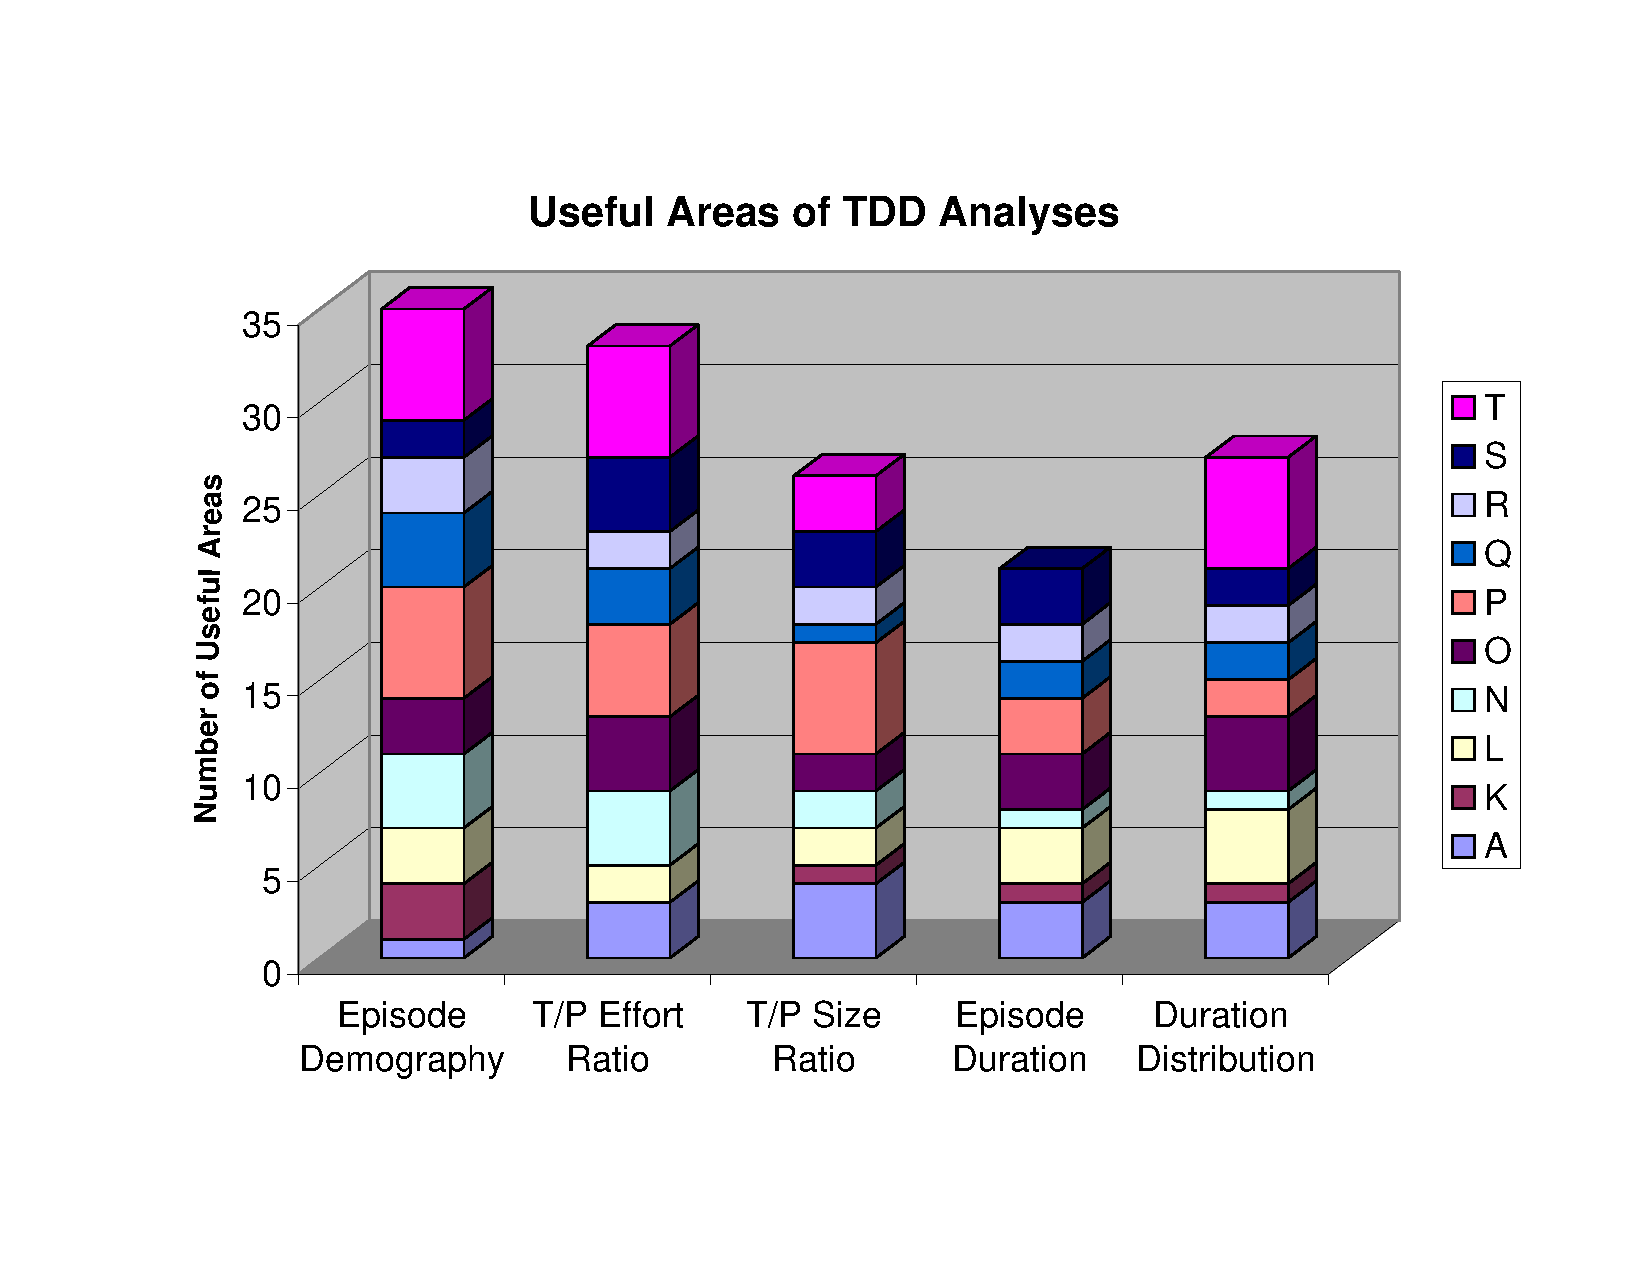
\includegraphics[width=1.0\textwidth]{figs/UsefulnessAreas}
  \caption{Useful Areas of TDD Analyses}
  \label{fig:3DUsefulnessAreas}
\end{figure}
With Figure \ref{fig:3DUsefulnessAreas}, we can easily compare the differences on usefulness among these 5 analyses. The ``Episode Demography'' and ``T/P Effort Ratio'' are the two most useful analyses. Although participants gave the least usefulness score to the ``Duration Distribution'' analysis, it has the potential to be useful basing upon its useful areas 

\subsubsection{Conclusion}
The analysis in this section provided supporting evidence to the research question Q2d. Participants generally agreed that the Zorro is useful and it can be used to understand and improve their TDD practices. %Note that there is a threat to the validity of this conclusion because usefulness evaluation is objective. %It is likely that the participants gave high scores because they did not want to offend me. In the industrial case study, I am going to evaluate it again. Since the participants in that study do not know me, they can freely give their opinions without worrying about being impolite.

\section{Chapter Summary}
\label{sec:discussion}
In this chapter, I validated Zorro's sensor data collection (sections \ref{subsec:SensorDataValidation}) and TDD behavior inference (\ref{subsec:VideoObservationValidation}). Based upon the participant observation analysis, these results provide supporting evidence to research questions Q2a and Q2b (See Chapter \ref{ch:Research}).

In this study, I used participant comments to cross-validate Zorro's inference of development behaviors and TDD compliance. The analysis of their comments (Section \ref{subsec:ParticipantCommentAnalysis}) provided supporting evidence to the research question Q2c. Participants cross-validated that Zorro inferred TDD development behaviors accurately and that participant observation is a reasonable research method for validating Zorro. 

As part of this study, I interviewed participants to survey their opinions on unit testing and TDD. The survey found that participants had a variety of opinions on how useful unit testing and 
TDD are (Section \ref{subsec:ParticipantInterviewAnalysis}). Most of them believed that unit testing and TDD can help to improve software quality. 

Participants also evaluated the usefulness of five TDD analyses provided by Zorro. The usefulness evaluation analysis (Section \ref{subsec:UsefulnessAnalysis}) found supporting evidence to the research question Q2d (See Chapter \ref{ch:Research}). 

In addition, I discovered an unexpected phenomenon (Section \ref{subsec:ParticipantGroup}) in the data analysis. Some participants sometimes forced Eclipse, the IDE I used in this study, to continue test invocations regardless of compilation errors. This behavior impacted Zorro's development stream partitioning and development behavioral inference. In this chapter's data analysis, I termed this development behavior as G2-DevBehavior, and divided participants into groups G1 and G2 for comparison. The validation analyses showed that Zorro's inference accuracy and consistency would improve significantly if Zorro could correctly interpret G2-DevBehavior. Thus it is necessary to let Zorro to allow this development behaviors in the future. 

%In sections \ref{subsec:VideoObservationValidation} and  \ref{subsec:ParticipantCommentAnalysis}, I discussed its effects using the video analysis and participant comment analysis. Even though Zorro yielded acceptable TDD behavior inference results, accommodating the G2-DevBehavior has the promise to improve Zorro's inference capability.